%!TEX TS-program = xelatex
\documentclass[12pt]{article}
\usepackage{geometry}
\geometry{verbose,letterpaper,tmargin=2.2cm,bmargin=2.2cm,lmargin=2.2cm,rmargin=2.2cm}
\usepackage[doublespacing]{setspace}
\usepackage[left]{lineno}
\renewcommand{\linenumberfont}{\normalfont\tiny}

% Figures at the end of the manuscript

% fonts
\usepackage{lmodern}

% authors and affiliations
\usepackage{authblk}
\renewcommand\Authfont{\scshape\normalsize}
\renewcommand\Affilfont{\itshape\small}

\usepackage{amssymb,amsmath}
\usepackage{ifxetex,ifluatex}
\ifnum 0\ifxetex 1\fi\ifluatex 1\fi=0 % if pdftex
  \usepackage[T1]{fontenc}
  \usepackage[utf8]{inputenc}
  \usepackage{textcomp} % provide euro and other symbols
\else % if luatex or xetex
  \usepackage{unicode-math}
  \defaultfontfeatures{Scale=MatchLowercase}
  \defaultfontfeatures[\rmfamily]{Ligatures=TeX,Scale=1}
\fi

% Use upquote if available, for straight quotes in verbatim environments
\IfFileExists{upquote.sty}{\usepackage{upquote}}{}
\IfFileExists{microtype.sty}{% use microtype if available
  \usepackage[]{microtype}
  \UseMicrotypeSet[protrusion]{basicmath} % disable protrusion for tt fonts
}{}
\makeatletter
\@ifundefined{KOMAClassName}{% if non-KOMA class
  \IfFileExists{parskip.sty}{%
    \usepackage{parskip}
  }{% else
    \setlength{\parindent}{0pt}
    \setlength{\parskip}{6pt plus 2pt minus 1pt}}
}{% if KOMA class
  \KOMAoptions{parskip=half}}
\makeatother
\usepackage{xcolor}
\IfFileExists{xurl.sty}{\usepackage{xurl}}{} % add URL line breaks if available
\IfFileExists{bookmark.sty}{\usepackage{bookmark}}{\usepackage{hyperref}}
\hypersetup{
  pdftitle={Sensitivity of tree species performance to climate and competition changes across their range distribution},
  pdfauthor={Willian~Vieira and Andrew~MacDonald and Dominique~Gravel},
  pdflang={en},
  pdfkeywords={Integral Projection Models, Perturbation
analysis, demography performance},
colorlinks=true,
allcolors=[rgb]{0,0.4,0.5},
pdfcreator={LaTeX via pandoc}}
\urlstyle{same} % disable monospaced font for URLs






\usepackage{graphicx}
\makeatletter
\def\maxwidth{\ifdim\Gin@nat@width>\linewidth\linewidth\else\Gin@nat@width\fi}
\def\maxheight{\ifdim\Gin@nat@height>\textheight\textheight\else\Gin@nat@height\fi}
\makeatother
% Scale images if necessary, so that they will not overflow the page
% margins by default, and it is still possible to overwrite the defaults
% using explicit options in \includegraphics[width, height, ...]{}
\setkeys{Gin}{width=\maxwidth,height=\maxheight,keepaspectratio}
% Set default figure placement to htbp
\makeatletter
\def\fps@figure{htbp}
\makeatother


\setlength{\emergencystretch}{3em} % prevent overfull lines
\providecommand{\tightlist}{%
  \setlength{\itemsep}{0pt}\setlength{\parskip}{0pt}}

\setcounter{secnumdepth}{5}




\newlength{\cslhangindent}
\setlength{\cslhangindent}{1.5em}
\newenvironment{cslreferences}%
  {\setlength{\parindent}{0pt}%
  \everypar{\setlength{\hangindent}{\cslhangindent}}\ignorespaces}%
  {\par}

\title{Sensitivity of tree species performance to climate and
competition changes across their range distribution}


\author[1]{Willian~Vieira\thanks{Corresponding author: willian.vieira@usherbrooke.ca}}
\author[1]{Andrew~MacDonald}
\author[1]{Dominique~Gravel}

\affil[1]{Département de biologie, Université de Sherbrooke, Sherbrooke,
QC, Canada}


\date{}

\linenumbers

\begin{document}

% print all title page only if not double-blind
\maketitle
\small{{\bf Running title}: Tree sensitivity to climate and
competition}\\\\
\small{{\bf Supporting information}: Additional supporting information can be found \href{https://willvieira.github.io/ms\_forest-ipm-sensitivity/suppInfo.pdf}{here}.}\\\\
\small{{\bf Acknowledgments}: We thank nice people}\\\\
\small{{\bf Data availability}: All the code and data used to reproduce
the analysis, figure and manuscript are stored as a research compendium
at \url{https://github.com/willvieira/ms_forest-ipm-sensitivity}).}\\\\
\small{{\bf Funding}: This research was supported by the BIOS² NSERC
CREATE program.}\\\\
\small{{\bf Conflicts of interest}: The authors declare no conflict of
interest.}\\\\
\begin{abstract}
Demographic range models, designed to scale individual variation to
predict population growth rate, offer a more mechanistic approach to
assessing species distribution than phenomenological models. Despite
numerous forest models adopting this approach to explore the influence
of climate and competition on species population growth rate, the
correlation of species performance with their distribution is often
weak. What remains unclear is whether the mismatch between species
performance and distribution arises from modelling limitations or if
climate and competition are poor predictors of species distribution.
Here, we developed an Integral Projection Model to evaluate the impact
of climate and competition on all demographic components of 31 tree
species from eastern North America. By using flexible nonlinear
hierarchical models, we filled most of the gaps in previous studies
while accounting for process uncertainty. Using perturbation analysis,
we found that population growth rate was more sensitive to mean annual
temperature than conspecific and heterospecific competition for all
species. Furthermore, we examined how population growth rate sensitivity
to climate and competition varied across the species range. The
dominance of climate over competition increased as species approached
the cold or hot temperature ranges. Moreover, most species exhibited a
decline in population growth rate sensitivity to competition from the
cold to the hot temperature range. Notably, the most influential
variable remained the local plot conditions captured by the random
effects. Unveiling species-specific sensitivity to climate and
competition provides crucial insights into how species may respond to
emerging conditions resulting from climate change and disturbance
changes.
\end{abstract}
\hspace{1cm}\small{{\bf Keywords}: Integral Projection
Models, Perturbation analysis, demography performance}



\hypertarget{introduction}{%
\section{Introduction}\label{introduction}}

The urge to unravel species distribution processes has increased with
the current global crisis, where 15 to 37\% of species are expected to
face extinction due to climate change (Thomas et al.
\protect\hyperlink{ref-thomas2004}{2004}). This urgency is particularly
pertinent for long-lived sessile species like trees, whose range
distribution is likely to fail to follow climate change (Zhu et al.
\protect\hyperlink{ref-Zhu2012}{2012}, Sittaro et al.
\protect\hyperlink{ref-Sittaro2017}{2017}). In an effort to enhance
traditional correlative species distribution models (e.g.~Guisan and
Zimmermann \protect\hyperlink{ref-Guisan2000}{2000}), theory decomposes
species distribution into smaller components to develop a more
mechanistic, process-based approach (Evans et al.
\protect\hyperlink{ref-Evans2016}{2016}). One such approach is
demographic range models, which predicts a species' distribution based
on individual performance determined by growth, survival, and
recruitment rates (Pagel and Schurr
\protect\hyperlink{ref-Pagel2012}{2012}). This approach operates under
the hypothesis that population growth rate (\(\lambda\)), determined by
demographic rates, varies across the environment, with the species range
limit defined by conditions where \(\lambda\) is positive (Maguire Jr
\protect\hyperlink{ref-maguire1973niche}{1973}, Holt
\protect\hyperlink{ref-Holt2009}{2009}). By approaching species
distribution from a demographic perspective, we can account for the
complexity of forest dynamics arising from multiple features such as
environment and species interaction (Schurr2012; Svenning et al.
\protect\hyperlink{ref-Svenning2014}{2014}).

Several studies have attempted to predict species distribution based on
demographic performance of forest trees. The most basic version of these
models uses environment-dependent demographic rates to predict
\(\lambda\) (e.g.~Merow et al. \protect\hyperlink{ref-Merow2014}{2014},
Csergő et al. \protect\hyperlink{ref-Csergo2017}{2017}). However,
factors like competition undeniably influence both demographic rates
(Clark et al. \protect\hyperlink{ref-Clark2011}{2011}, Luo and Chen
\protect\hyperlink{ref-Luo2011}{2011}, Zhang et al.
\protect\hyperlink{ref-Zhang2015}{2015}) and population performance
(Scherrer et al. \protect\hyperlink{ref-Scherrer2020}{2020}, Le Squin et
al. \protect\hyperlink{ref-LeSquin2021}{2021}) in forest trees. This
realized version of the niche (Hutchinson
\protect\hyperlink{ref-Hutchinson1957}{1957}) may explain why North
American forest trees often do not occur within their climatically
suitable range (Boucher-Lalonde et al.
\protect\hyperlink{ref-BoucherLalonde2012}{2012}, Talluto et al.
\protect\hyperlink{ref-Talluto2017}{2017}).

An increasing body of evidence conflicts with theoretical expectations
by observing weak correlations between the demographic performance of
trees and their distribution (McGill
\protect\hyperlink{ref-McGill2012}{2012}, Csergő et al.
\protect\hyperlink{ref-Csergo2017}{2017}, Bohner and Diez
\protect\hyperlink{ref-bohner2020}{2020}, Le Squin et al.
\protect\hyperlink{ref-LeSquin2021}{2021}, Midolo et al.
\protect\hyperlink{ref-Midolo2021}{2021}, Guyennon et al.
\protect\hyperlink{ref-Guyennon2023}{2023}, Thuiller et al.
\protect\hyperlink{ref-Thuiller2014}{2014}). This mismatch is often
attributed to the oversight of processes beyond climate and competition.
For instance, habitat availability coupled with dispersal limitations
can restrict a species' distribution even in locations where performance
is positive (Pulliam \protect\hyperlink{ref-Pulliam2000}{2000}).
However, the precision of methods used to quantify demographic
performance is rarely challenged, perhaps in part because each attempt
employs a different approach. Some studies assess performance based
solely on one of the growth, survival, or recruitment rates (McGill
\protect\hyperlink{ref-McGill2012}{2012}, Bohner and Diez
\protect\hyperlink{ref-bohner2020}{2020}). When demographic rates are
integrated into population models, specific components, such as
recruitment, are often overlooked due to data limitations (Kunstler et
al. \protect\hyperlink{ref-Kunstler2021}{2021}, Le Squin et al.
\protect\hyperlink{ref-LeSquin2021}{2021}). Moreover, some studies do
not account for density dependence (Csergő et al.
\protect\hyperlink{ref-Csergo2017}{2017}, Ohse et al.
\protect\hyperlink{ref-Ohse2023}{2023}), and when they do, they rarely
differentiate between conspecific and heterospecific competition (Bohner
and Diez \protect\hyperlink{ref-bohner2020}{2020}, Le Squin et al.
\protect\hyperlink{ref-LeSquin2021}{2021}). Finally, despite the need to
embrace model and data uncertainty (Milner-Gulland and Shea
\protect\hyperlink{ref-MilnerGulland2017a}{2017}), most of these studies
assessed performance under average covariate conditions and pointwise
estimations, neglecting the associated uncertainty of the estimates.

Rather than asking whether demographic performance correlates with
distribution, a more fruitful question may be how climate and
competition influence demographic performance. Indeed, we still miss a
comprehensive partitioning of the sensitivity of forest dynamics to
local and biogeographical drivers of performance (Ohse et al.
\protect\hyperlink{ref-Ohse2023}{2023}). For instance, Clark et al.
(\protect\hyperlink{ref-Clark2011}{2011}) found that annual growth rate
is more sensitive to competition, while fecundity is more sensitive to
climate. In contrast, Copenhaver-Parry and Cannon
(\protect\hyperlink{ref-CopenhaverParry2016}{2016}) found that growth
was more sensitive to climate than competition. These studies provide
crucial insights into how forest trees will respond to climate change
and forest management, supporting conservation planning. However, they
only assess the importance of climate and competition on single
demographic components, lacking a complete picture of population
dynamics. This is especially critical if species are susceptible to
variation in sensitivity to climate and competition across life history
stages (Russell et al. \protect\hyperlink{ref-Russell2012}{2012},
Ettinger and HilleRisLambers
\protect\hyperlink{ref-Ettinger2013}{2013}). Furthermore, the
sensitivity of \(\lambda\) to climate and competition may depend on the
species range position, such as climate being relatively more important
in abiotic stressful conditions and competition being more critical when
climate is benign (Louthan et al.
\protect\hyperlink{ref-Louthan2015}{2015}). Nevertheless, such
information is still lacking for trees (Ohse et al.
\protect\hyperlink{ref-Ohse2023}{2023}).

Here, we evaluate how climate and competition affect the demography and
population growth rate of the 31 most abundant forest tree species
across Eastern North America. We leverage the complete (26 - 53°)
latitudinal coverage of forest inventories across the US and Canada to
capture the entire range of these species. Specifically, we model each
of the growth, survival, and recruitment vital rates as a function of
mean annual temperature and precipitation, as well as conspecific and
heterospecific basal area density, serving as a proxy for competition
for light. We fit these demographic models with a flexible, non-linear
hierarchical Bayesian model. The non-linear approach captures both the
complexity of trees' demographic rates and the multiple-effect forms of
climate and competition. Furhtermore, the hierarchical Bayesian approach
allows one to account for model uncertainty at different organizational
scales. These demographic rate models are then incorporated into a
size-structured Integral Projection Model (IPM) to quantify the
\(\lambda\) of each species under climate and competition effects.

Our primary goal is to use the fitted IPM to compute the sensitivity of
each species' \(\lambda\) to climate and competition across their range.
Employing perturbation analysis, we quantify the relative contribution
of each covariate to changes in \(\lambda\) (Caswell
\protect\hyperlink{ref-Caswell2000}{2000}). Precisely, we assess the
species sensitivity of an observed \(\lambda\) for each plot-year
combination based on their specific climate and competition conditions.
This approach enables an evaluation of the overall sensitivity of
\(\lambda\) to a covariate while considering the inherent variability of
the covariate experienced by the species. For instance, a species may
exhibit high sensitivity to temperature, but if most of its distribution
is observed under optimal temperature conditions, the average
sensitivity of the species will be low.

Lastly, expanding on previours findings indicating the inability of
North American trees to both expand their cold range and contract their
hot range under climate change (Talluto et al.
\protect\hyperlink{ref-Talluto2017}{2017}), we ask if sensitivity to
climate and competition changes across the species' cold and hot ranges.
Furthermore, we explore whether the relative sensitivity between climate
and competition changes across the species' distribution range. Our
integrative approach allows us to assess the relative effects of climate
and competition from demographic rates up to the population growth rate
while accounting for model uncertainties and stand structure, revealing
essential insights into understanding the response of forest trees to
climate change, management practices, and conservation efforts.

\hypertarget{methods}{%
\section{Methods}\label{methods}}

\hypertarget{forest-inventory-and-climate-data}{%
\subsection{Forest inventory and climate
data}\label{forest-inventory-and-climate-data}}

We used two open inventory datasets from eastern North America: the
Forest Inventory and Analysis (FIA) dataset in the United States
(O'Connell et al. \protect\hyperlink{ref-OConnell2007}{2007}) and the
Forest Inventory of Québec (Minist\a`ere des Ressources Naturelles
\protect\hyperlink{ref-Naturelles2016}{2016}). At the plot level, we
focused on plots sampled at least twice, excluding those that had
undergone harvesting to concentrate solely on natural dynamics.
Specifically, we selected surveys conducted for the FIA dataset using
the modern standardized methodology implemented since 1999. After
applying these filters, our final dataset encompassed nearly 26,000
plots spanning a latitude range from 26° to 53° (Figure S7). Each plot
within the dataset was measured between 1970 and 2021, with observation
frequencies ranging from 2 to 7 times and an average of 3 measurements
per plot. The time intervals between measurements varied from 1 to 40
years, with a median interval of 7 years (Figure S7).

These datasets provide individual-level information on the diameter at
breast height (DBH) and the status (dead or alive) of more than 200
species. From this pool, we selected the 31 most abundant species (Table
S1). This selection comprises 9 conifer species and 22 hardwood species.
We ensured an even distribution of species across the shade tolerance
axis, with three species classified as very intolerant, nine as
intolerant, eight as intermediate, eight as tolerant, and five as very
tolerant (Burns et al. \protect\hyperlink{ref-burns1990silvics}{1990}).

For the competition metric, we use asymmetric competition for light,
meaning that each individual is affected only by neighbour individuals
of larger size. We quantified asymmetric competition for light for a
focal individual in a given plot by summing the total basal area of all
individuals larger than the focal one, herein BAL. We further split BAL
into the total density of conspecific and heterospecific individuals.
For the climate variable, we obtained the 19 bioclimatic variables with
a 10 \(km^2\) (300 arcsec) resolution grid, covering the period from
1970 to 2018. These climate variables were modeled using the ANUSPLIN
interpolation method (McKenney et al.
\protect\hyperlink{ref-McKenney2011}{2011}). We used each plot's
latitude and longitude coordinates to extract the mean annual
temperature (MAT) and mean annual precipitation (MAP). In cases where
plots did not fall within a valid pixel of the climate variable grid, we
interpolated the climate condition using the eight neighboring cells.
Due to the transitional nature of the dataset, we considered both the
average and standard deviation of MAT and MAP over the years within each
time interval.

\hypertarget{model}{%
\subsection{Model}\label{model}}

We evaluated the population growth rates of the 31 forest species using
an Integral Projection Model (IPM). An IPM is a mathematical tool used
to represent the dynamics of structured populations and communities. It
distinguishes itself from traditional population models with the
representation of a continuous trait in discrete time (Easterling et al.
\protect\hyperlink{ref-Easterling2000}{2000}). This is especially
relevant for trees due to the considerable variability in demographic
rates depending on individual size (Kohyama
\protect\hyperlink{ref-kohyama1992}{1992}). Specifically, the IPM
consists of a set of functions predicting the transition of a
distribution of individual traits from time \(t\) to time \(t+1\):

\begin{equation}
n(z', t + 1) = \int_{L}^{U} \, K(z', z, \theta)\, n(z, t)\, \mathrm{d}z
\label{eq:ipm}\end{equation}

The continuous trait \(z\) at time \(t\) represents the DBH, bouded
between the lower (\(L\)) and upper (\(U\)) values, and \(n(z, t)\)
characterizes the continuous DBH distribution for a population. The
probability of the population distribution size from \(n(z, t)\) to
\(n(z', t+1)\) is governed by the kernel \(K\) and the species-specific
parameters \(\theta\). The kernel \(K\), a continuous version of the
discretized projection Matrix in structured population models, is
composed of three sub-models:

\begin{equation}
K(z', z, \theta) = [Growth(z', z, \theta) \times Survival(z, \theta)] + Recruitment(z, \theta)
\label{eq:kernel}\end{equation}

The growth function describes how individual trees increase in size,
while the survival function determines the probability of staying alive
throughout the next time step. The recruitment model describes the
number of individuals ingressing the population. Below, we describe the
basic (intercept) version of these models, followed by the inclusion of
each climate and competition covariate.

\hypertarget{demographic-rates}{%
\subsubsection{Demographic rates}\label{demographic-rates}}

\textbf{Growth} - the size in DBH of an individual at time
\(t + \Delta t\) after growing from time \(t\) is determined by:

\begin{equation}
  dbh_{i,t + \Delta t} \sim N(\mu_{i, t+\Delta t}, \sigma)
\label{eq:VBlik}\end{equation}

We used the von Bertalanffy growth equation to describe the annual
growth rate in DBH of an individual \(i\) (Von Bertalanffy
\protect\hyperlink{ref-von1957quantitative}{1957}). The average size at
time \(t+\Delta t\) from the initial size \(dbh_{i, t}\) of an
individual at time \(t\) is given by:

\begin{equation}
  \mu_{i, t+\Delta t} = dbh_{i,t}  \times e^{-\Gamma \Delta t} + \zeta_{\infty} (1- e^{-\Gamma \Delta t})
\label{eq:VBmodel}\end{equation}

Where \(\Delta t\) is the time interval between the initial and final
size measurements and \(\Gamma\) represents a dimensionless growth rate
coefficient. \(\zeta_{\infty}\) denotes the asymptotic size, which is
the location at which growth approximates to zero. The rationale behind
this model is that the growth rate exponentially decreases with size,
converging to zero as size approaches \(\zeta_{\infty}\). This
assumption is particularly valuable in the context of the IPM, as it
prevents eviction --- where individuals are projected beyond the limits
of the size distribution (\([L, U]\)) defined by the Kernel.

\textbf{Survival} - The chance of a mortality event (\(M\)) for an
individual \(i\) within the time interval between \(t\) and
\(t+\Delta t\) is modeled as a Bernoulli distribution:

\begin{equation}
M_i \sim Bernoulli(p_i)
\label{eq:survL}\end{equation}

Here, \(M_i\) represents the individual's status (alive/dead) and
\(p_i\) the mortality probability of the individual \(i\). The mortality
probability is calculated based on the annual survival rate (\(\psi\))
and the time interval between census (\(\Delta t\)):

\begin{equation}
p_i = 1 - \psi^{\Delta t}
\label{eq:survP}\end{equation}

The model assumes that the survival probability (\(1 - p_i\)) increases
with the longevity parameter \(\psi\), but is compensated exponentially
with the increase in time \(\Delta t\).

\textbf{Recruitment} - We combined data from the U.S. and Quebec forest
inventories to obtain a broader range of climatic conditions. However,
these inventories have inconsistent protocols for recording seedlings,
saplings, and juveniles. Most of all, they have different size
thresholds for individual-based measurements. Therefore, we quantified
the recruitment rate (\(I\)) as the ingrowth of new individuals into the
adult population, defined as those with a DBH exceeding 12.7 cm. The
quantity \(I\) encompasses the processes of fecundity, dispersal,
growth, and survival up to reaching the size threshold. Similar to
growth and survival, the count of ingrowth individuals (\(I\)) reaching
the 12.7 cm size threshold depends on the time interval between
measurements. We introduce two parameters to control the potential
number of recruited individuals: \(\phi\), determining the annual
ingrowth rate per square meter, and \(\rho\), denoting the annual
survival probability of each ingrowth individual:

\begin{equation}
  I \sim Poisson(~\phi \times A \times \frac{1 - \rho^{\Delta t}}{1-\rho}~)
\label{eq:rec}\end{equation}

Where \(A\) represents the area of the plot in square meters. The model
assumes that new individuals enter the population annually at a rate of
\(\phi\), and their likelihood of surviving until the subsequent
measurement (\(\rho\)) declines over time. Note that \(\rho\) in
Equation \ref{eq:rec} is not associated with Equation \ref{eq:survP}
determining the survival of the adults. Instead, \(\rho\) is estimated
from the data of individuals arriving in the population. Once an
individual is recruited into the population, a submodel determines its
initial size \(z_I\), increasing linearly with time:

\begin{equation}
  z_{I} \sim TNormal(\Omega + \beta \Delta t,~\sigma, ~ \alpha, ~ \beta)
\label{eq:recSize}\end{equation}

The \(TNormal\) is a truncated distribution with lower and upper limits
determined by the \(\alpha\) and \(\beta\) parameters, respectively. We
set \(\alpha\) to 12.7 cm, aligning it with the ingrowth threshold,
while \(\beta\) is set to infinity to allow for an unbounded upper
limit.

\hypertarget{covariates}{%
\subsubsection{Covariates}\label{covariates}}

\textbf{Random effects} - We introduced plot-level random effects in
each of the growth, survival, and recruitment demographic component to
account for shared variance between the individuals within the same
plot. For a demographic component with an average intercept
\(\overline{I}\), an offset value (\(\alpha\)) is drawn for each plot
\(j\) from a normal distribution with a mean of zero and variance
\(\sigma\):

\begin{equation}
\begin{split}
&\alpha_{j} \sim N(0, \sigma) \\[2pt]
&I_j = \overline{I} + \alpha_j
\end{split}
\label{eq:randomEffect}\end{equation}

Where \(\sigma\) represents the variance among all plots \(j\) and \(I\)
can take one of three forms: \(\Gamma\) for growth, \(\psi\) for
survival, and \(\phi\) for the recruitment model.

\textbf{Competition} - We used basal area of larger individuals (BAL;
asymmetric competition) instead of total basal area (BA; symmetric
competition), assuming that competition for light is the primary
competitive factor driving forest dynamics (Pacala et al.
\protect\hyperlink{ref-Pacala1996a}{1996}). Therefore, each of the
growth (\(\Gamma\)), longevity (\(\psi\)), and recruitment survival
(\(\rho\)) parameters decreases exponentially with BAL. Take \(I\) as
one of the three parameters, the effect of BAL on \(I\) is driven by two
parameters describing the conspecific (\(\beta\)) and heterospecific
(\(\theta\)) competition:

\begin{equation}
  I + \beta (BAL_{cons} + \theta \times BAL_{het})
\label{eq:compEffect}\end{equation}

When \(\theta < 1\), conspecific competition is stronger than
heterospecific competition. Conversely, heterospecific competition
prevails when \(\theta > 1\), and when \(\theta = 1\), there is no
distinction between conspecific and heterospecific competition. Note
that \(\beta\) is also unbounded, allowing it to converge towards
negative (indicating competition) or positive (indicating facilitation)
values. Furthermore, we fixed \(\theta = 1\) for the recruitment
(\(I = \rho\)) due to model convergence issues. The recruitment model
also accounts for the conspecific density dependence effect on the
annual ingrowth rate (\(\phi\)). Specifically, \(\phi\) increases with
\(BAL_{cons}\) as a positive effect of seed source up to reach the
optimal density of recruitment, \(\delta\), where it then decreases with
more conspecific density due to competition at a rate proportional to
\(\sigma\):

\begin{equation}
  \phi + \left(\frac{BAL_{cons} - \delta}{\sigma}\right)^2
\label{eq:compingrowth}\end{equation}

\textbf{Climate} - We selected mean annual temperature (MAT) and mean
annual precipitation (MAP) bioclimatic variables as they are widely used
in species distribution modeling and were previously found relevant to
model demography of these species (Le Squin et al.
\protect\hyperlink{ref-LeSquin2021}{2021}). Each demographic component
\(I\), representing either \(\Gamma\) for growth, \(\psi\) for
longevity, or \(\phi\) for ingrowth, varies as a bell-shaped curve
determined by an optimal climate condition (\(\xi\)) and a climate
breadth parameter (\(\sigma\)):

\begin{equation}
  I + \left(\frac{MAT - \xi_{MAT}}{\sigma_{MAT}}\right)^2 + \left(\frac{MAP - \xi_{MAP}}{\sigma_{MAP}}\right)^2
\label{eq:compEffect}\end{equation}

The climate breadth parameter (\(\sigma\)) influences the strength of
the specific climate variable's effect on each demographic component.
This unimodal function is flexible, assuming various shapes, such as
bell, quasi-linear, or flat shapes. However, this flexibility introduces
the possibility of parameter degeneracy or redundancy, where different
combinations of parameter values yield similar outcomes. To address this
issue, we constrained the optimal climate condition parameter (\(\xi\))
within the observed climate range for the species, assuming that the
optimal climate condition falls within our observed data range.

\hypertarget{model-fit-and-validation}{%
\subsubsection{Model fit and
validation}\label{model-fit-and-validation}}

We fitted each of the growth, survival, and recruitment models
separately for each species, using the Hamiltonian Monte Carlo (HMC)
algorithm implemented in the Stan software (version 2.30.1 Team and
Others \protect\hyperlink{ref-stan2022stan}{2022}) with the
\texttt{cmdstandr} R package interface (version 0.5.3 Gabry et al.
\protect\hyperlink{ref-cmdstanr}{2023}). We conducted 2000 iterations
for the warm-up and 2000 iterations for the sampling phase for each of
the four chains, resulting in 8000 posterior samples (excluding the
warm-up). However, we kept only the last 1000 iterations of the sampling
phase to save computation time and storage space, resulting in 4000
posterior samples. We build and fit each demographic component
incrementally, from a simple intercept, and gradually incorporate plot
random effects, competition, and climate covariates. Recall that our
goal is not to have the most complex model to achieve the highest
predictive metric but to make inferences (Tredennick et al.
\protect\hyperlink{ref-Tredennick2021}{2021}). We focus on assessing the
relative effects of climate and competition while controlling for other
influential factors. Therefore, our modeling approach is guided by
biological mechanisms, which tend to provide more robust extrapolation
(Briscoe et al. \protect\hyperlink{ref-Briscoe2019}{2019}) rather than
being solely dictated by specific statistical metrics. Nevertheless, we
checked if increasing model complexity with new covariates does not
result in worse performance using complementary metrics such as mean
squared error (MSE), pseudo \(R^2\) (Gelman et al.
\protect\hyperlink{ref-Gelman2019}{2019}), and Leave-One-Out
Cross-Validation (LOO-CV). Detailed discussions regarding model fit,
diagnostics, and model comparison can be found in supplementary material
1.

With the fitted demographic components, we constructed the Kernel \(K\)
of the IPM following Equation \ref{eq:kernel}. We employed the mid-point
rule to perform the discrete-form integration of the continuous \(K\)
(Ellner et al. \protect\hyperlink{ref-Ellner2016}{2016}). This involved
discretizing the projection kernel \(K\) using bins of 0.1 cm, which are
considered appropriate for obtaining unbiased estimates (Zuidema et al.
\protect\hyperlink{ref-zuidema2010integral}{2010}). Finally, we computed
the asymptotic population growth rate (\(\lambda\)) using the leading
eigenvalue of the discretized matrix \(K\).

\hypertarget{perturbation-analysis}{%
\subsection{Perturbation analysis}\label{perturbation-analysis}}

We use perturbation analysis to assess the sensitivity of \(\lambda\) to
competition and climate conditions (Caswell
\protect\hyperlink{ref-Caswell2000}{2000}). We define sensitivity as the
partial derivative of \(\lambda\) with respect to a covariate \(X\),
which can take the form of either conspecific or heterospecific density
dependence competition, or temperature or precipitation climate
conditions. In practice, we quantify sensitivity by slightly increasing
each covariate value \(X_j\) to \(X_j^{'}\) and computing the change in
\(\lambda\) following the right-hand part of Equation \ref{eq:sens}:

\begin{equation}
    \frac{\partial \lambda_{ij}}{\partial X_j} \bigg\rvert_{K_{ij}} \approx \frac{\Delta \lambda_{ij}}{\Delta X_j} = \frac{|f(X_j^{'}) - f(X_j)|}{X_j^{'} - X_j}
\label{eq:sens}\end{equation}

Sensitivity is evaluated separately for each species \(i\) and is
conditional on the specific climate and competition conditions observed
for the plot \(j\), along with the Kernel \(K_{ij}\) parameters. We set
the perturbation size to a 1\% increase in the normalized scale for each
covariate. For instance, a 1\% increase translates to a rise of 0.3°C
for Mean Annual Temperature (MAT) and 26 mm for Mean Annual
Precipitation (MAP). Because the competition metric is computed at the
individual level, the perturbation was applied to each individual, where
a 1\% increase corresponds approximately to a rise of 1.2 cm in dbh. As
we were interested in the absolute difference, the resulting sensitivity
value ranges between 0 and infinity, with lower values indicating a
lower sensitivity of \(\lambda\) to the specific covariate. We computed
the log ratio between competition and climate (\(CCR\)) sensitivities to
discern their relative effects as follows:

\begin{equation}
\begin{split}
&S_{comp, ij} = \frac{\partial \lambda_{ij}}{\partial BA_{cons, i}} + \frac{\partial \lambda_{ij}}{\partial BA_{het, i}} \\[2pt]
&S_{clim, ij} = \frac{\partial \lambda_{ij}}{\partial MAT_{i}} + \frac{\partial \lambda_{ij}}{\partial MAP_{i}} \\[2pt]
&CCR_{ij} = \text{ln} \frac{S_{comp, ij}}{S_{clim, ij}}
\end{split}
\label{eq:CCR}\end{equation}

Here, \(S\) represents the total sensitivity of species \(i\) to
competition or climate for a given plot \(j\). Negative \(CCR\) values
indicate higher sensitivity of \(\lambda\) to climate, while positive
values indicate the opposite.

When averaging \(S_{X,i}\) across \(j\), this metric reflects the
sensitivity of \(\lambda_i\) to \(X\), which is conditional upon the
probability distribution of the covariate \(X\). We categorized each
plot into cold, center, or hot conditions along the MAT axis for every
species. Plots were labeled as cold (or hot) if the average MAT fell
below (above) the 10\% (90\%) probability distribution, with all
intermediate plots considered center plots. Thus, sensitivity to a
covariate in the cold range of the species signifies the average
sensitivity among all plots classified as cold. It is important to note
that this classification is also conditional on the probability
distribution of observed MAT within the species.

The code to fit each demographic component is available in the
\href{https://github.com/willvieira/TreesDemography}{\texttt{TreesDemography}}
GitHub repository. The code for the IPM model and the respective
sensitivity analysis is available in the
\href{https://github.com/willvieira/forest-IPM/tree/master/simulations/covariates_perturbation}{\texttt{forest-IPM}}
GitHub repository.

\hypertarget{results}{%
\section{Results}\label{results}}

\hypertarget{model-validation}{%
\subsection{Model validation}\label{model-validation}}

All species-specific demographic components demonstrated convergence
with \(\hat{R} <1.05\) and low to no divergent iterations. In comparing
the simple intercept model with the more complete versions, the LOO-CV
consistently favored the complete model for all three demographic rates,
featuring plot random effects, competition, and climate covariates, over
other competing models (supplementary material 1). The absolute values
of LOO-CV suggested that the growth model gained the most information
from including covariates, followed by recruitment and survival models.
We further validated our model predictions by comparing the parameters
with traits groups such as growth rate classes, maximum observed size,
maximum observed age, shade tolerance, and seed mass (Burns et al.
\protect\hyperlink{ref-burns1990silvics}{1990}, Díaz et al.
\protect\hyperlink{ref-diaz2022}{2022}).

The growth model intercept comprises two parameters, one determining the
asymptotic size (\(\zeta_{\infty}\)) and the annual growth rate
\(\Gamma\). The \(\zeta_{\infty}\) can be interpreted as the maximum
predicted size of the species, which correlates well across all 31
species with the maximum observed size in the literature
(\(R^2 = 0.31\), Figure \ref{fig:crossGrowthSurv}). Similarly,
\(\Gamma\) among the species exhibited a distribution aligning with the
fast, moderate, and slow-growing traits (Figure S8). In the survival
model, the expected longevity (\(L\)) can be derived from the annual
survival rate ( \(\psi\)) following the equality \(L = e^{\psi}\),
showing a high correlation with the maximum observed age in the
literature (\(R^2 = 0.59\), Figure \ref{fig:crossGrowthSurv}). In the
recruitment model, the log of the annual ingrowth rate (\(\phi\))
reduced linearly with seed mass (Figure S9), capturing the seed
mass-growth rate tradeoff (Reich et al.
\protect\hyperlink{ref-Reich1998}{1998}). Additionally, the annual
survival probability of ingrowth (\(\rho\)) decreased with intolerance
to shade (Figure S10).

\begin{figure}
\hypertarget{fig:crossGrowthSurv}{%
\centering
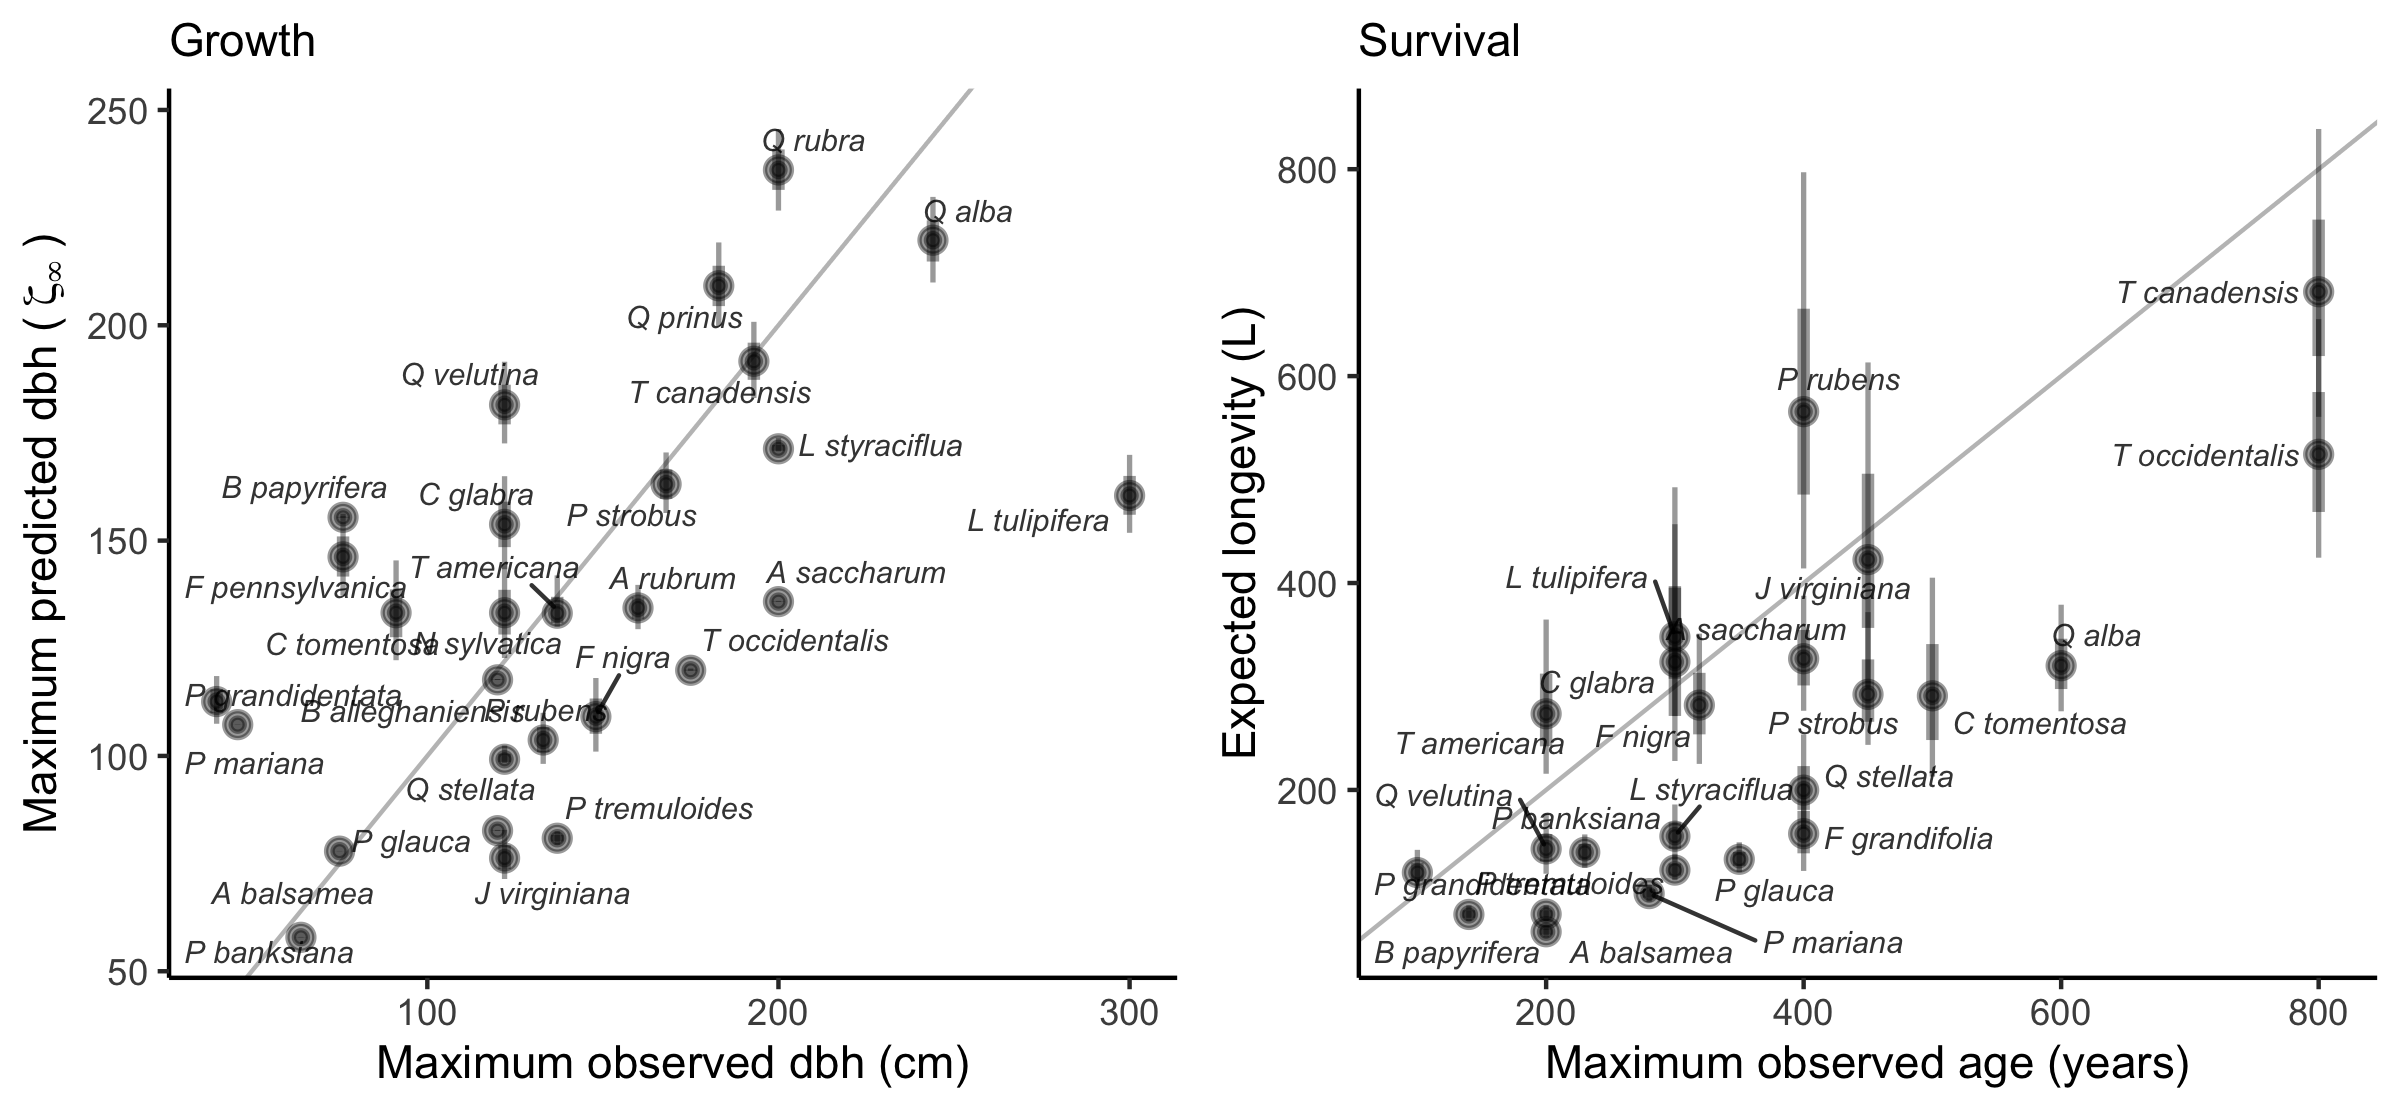
\includegraphics[width=1\textwidth,height=\textheight]{manuscript/figs/crossGrowthSurv.png}
\caption{Correlation between predicted asymptotic size
(\(\zeta_{\infty}\)) with maximum observed size (left) and predicted
longevity (\(L\)) with maximum observed age for the 31 forest species.
Maximum observed size and age are obtained from Burns et al.
(\protect\hyperlink{ref-burns1990silvics}{1990}). The gray line is the
identity curve.}\label{fig:crossGrowthSurv}
}
\end{figure}

Both conspecific and heterospecific competition effects for the growth
and survival models increased with intolerance to shade (Figure
\ref{fig:crossComp}). The stronger competition effect of conspecific
over heterospecific was consistent for almost all species in both growth
and survival models. Only two species for growth and three for survival
among the 31 presented stronger heterospecific competition than
conspecific competition. Moreover, \emph{Fagus grandifolia} and
\emph{Thuja occidentalis} exhibited positive density dependence for the
survival model. For recruitment, the effect of total stand density
increased with shade intolerance among the species (Figure S11).

\begin{figure}
\hypertarget{fig:crossComp}{%
\centering
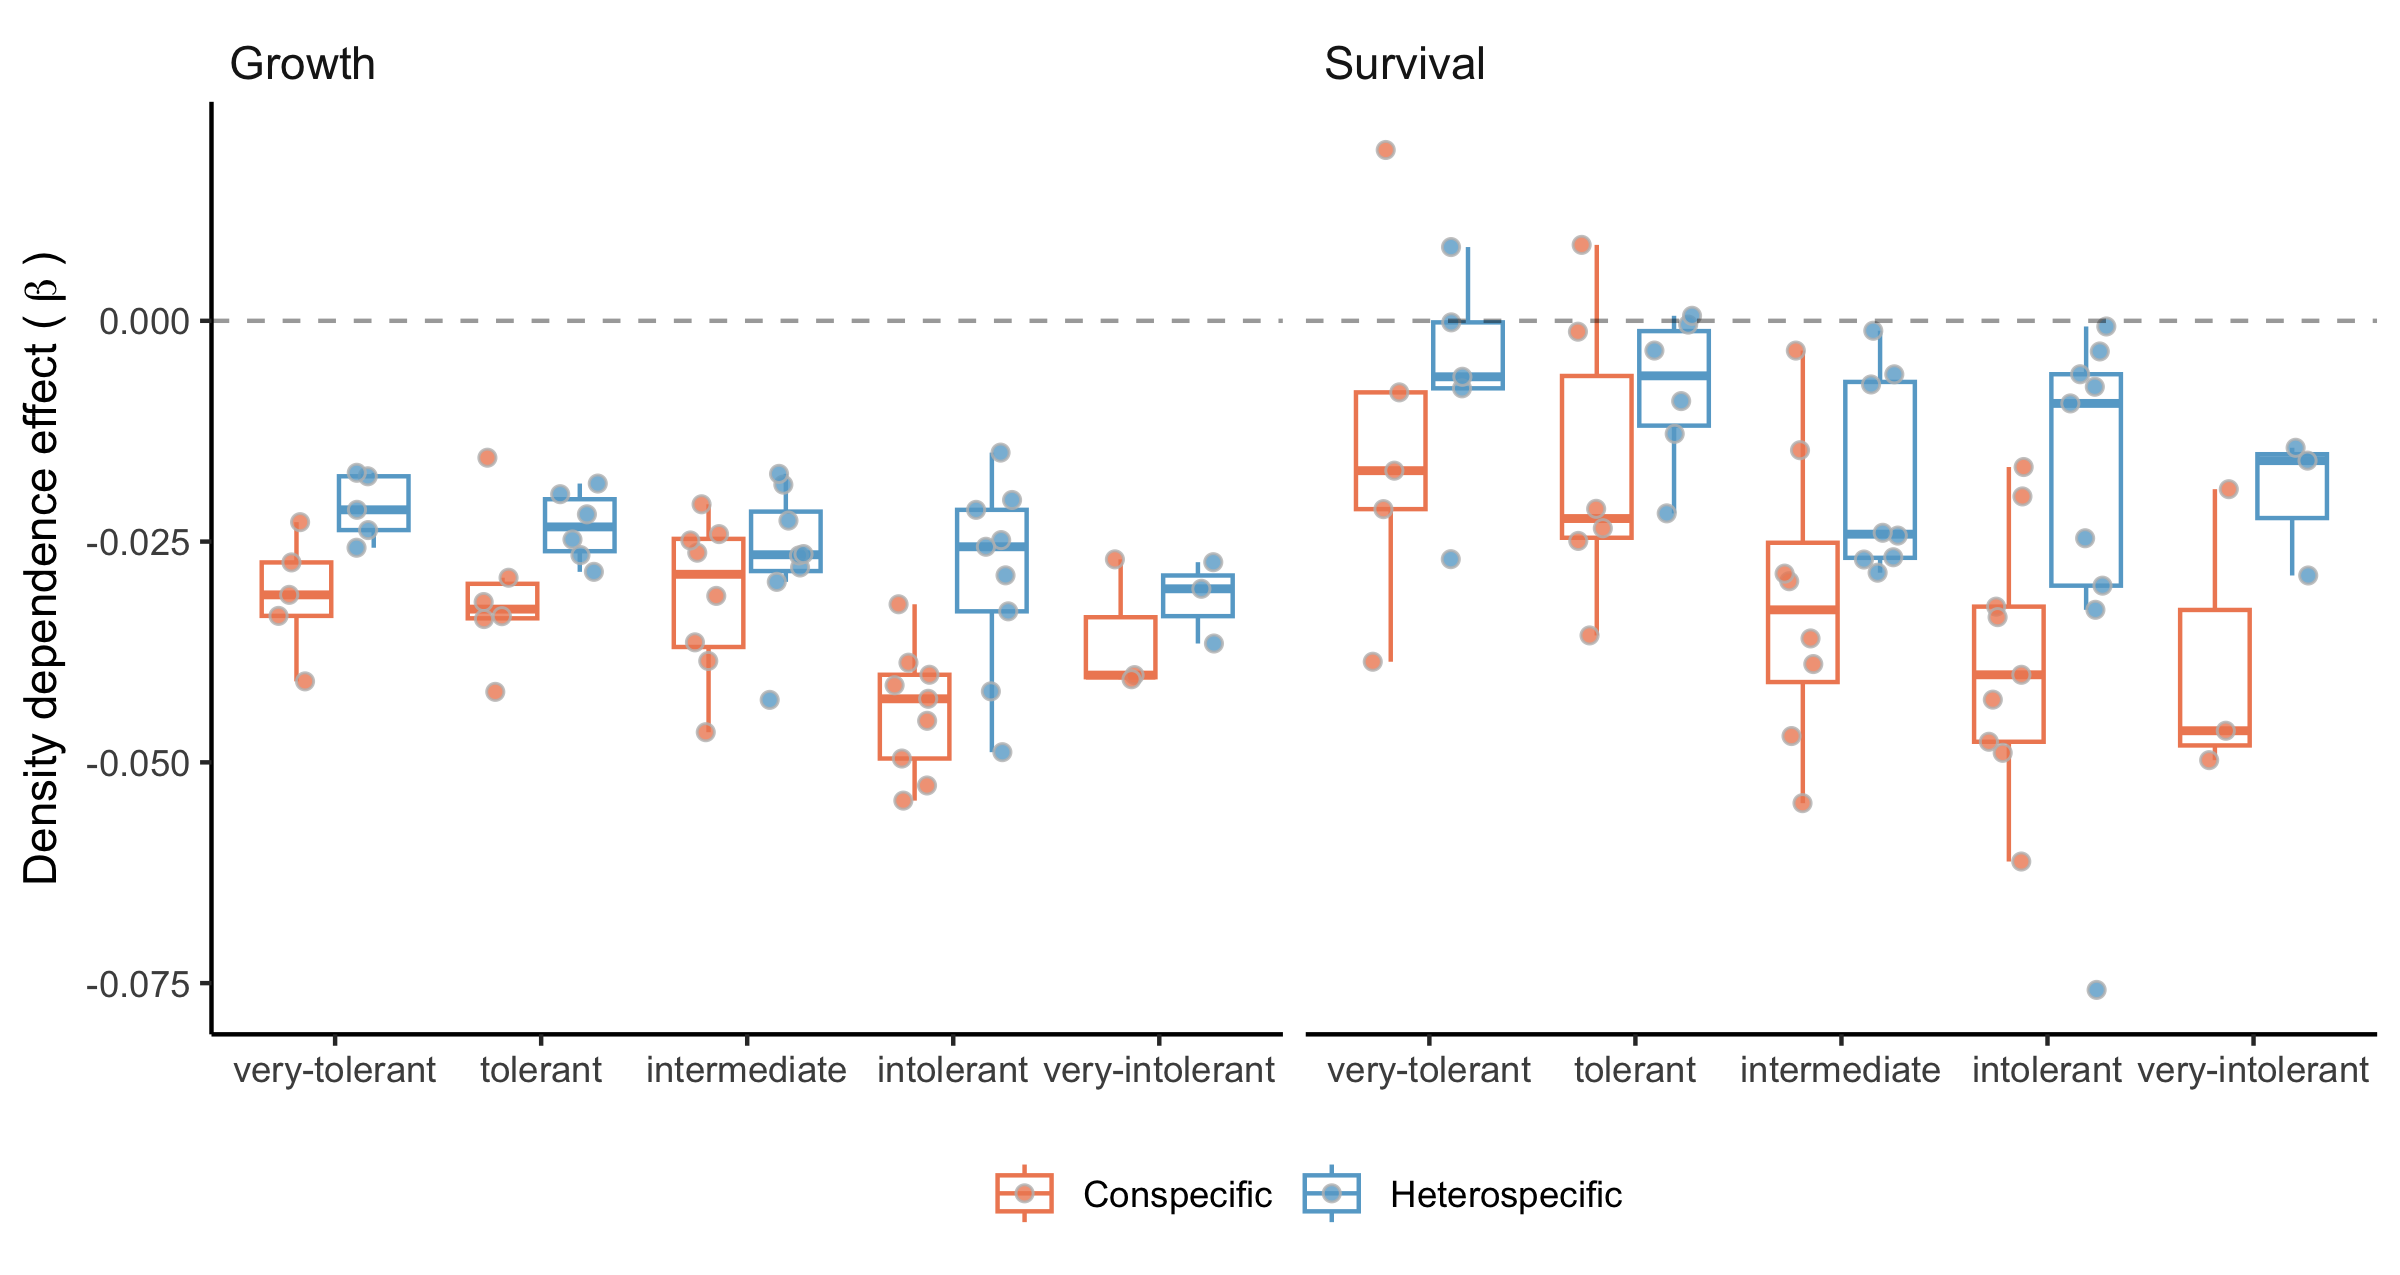
\includegraphics[width=1\textwidth,height=\textheight]{manuscript/figs/crossComp.png}
\caption{Posterior distribution for the conspecific (red) and
heterospecific (blue) density dependence for each class of shade
tolerance (Burns et al. \protect\hyperlink{ref-burns1990silvics}{1990}).
The more negative the \(\beta\), the stronger the competition
effect.}\label{fig:crossComp}
}
\end{figure}

The distribution of optimal MAT (\(\xi_{MAT}\)) and MAP (\(\xi_{MAP}\))
for the 31 species revealed that the optimal climates for growth,
survival, and recruitment were rarely located at the center of the
species ranges (Figure S12 and S13). Furthermore, most species exhibited
some degree of demographic compensation, that is, opposing responses to
the environment between demographic rates (Villellas et al.
\protect\hyperlink{ref-Villellas2015}{2015}). Lastly, the climate
breadth (\(\sigma\)) determined how flat or narrow the performance of
species was across MAT and MAP. We found among all species that climate
breadth increased with range size, demonstrating that species with more
range occupancy had larger niche breadths. The exception was the niche
breadth of survival over MAT, showing a weak, flat correlation.

\hypertarget{lambda-sensitivity-to-climate-and-competition}{%
\subsection{\texorpdfstring{\(\lambda\) sensitivity to climate and
competition}{\textbackslash lambda sensitivity to climate and competition}}\label{lambda-sensitivity-to-climate-and-competition}}

We used perturbation analysis to assess the relative contribution of
each covariate to changes in \(\lambda\). Figure \ref{fig:mean_sens}
describes the average sensitivity of each species' population growth
rate to conspecific and heterospecific competition, temperature, and
precipitation. Across all species, \(\lambda\) exhibited higher
sensitivity to temperature, followed by conspecific and heterospecific
competition, while sensitivity to mean annual precipitation was
practically zero. This observation of sensitivity to the covariates was
consistent across all species.

\begin{figure}
\hypertarget{fig:mean_sens}{%
\centering
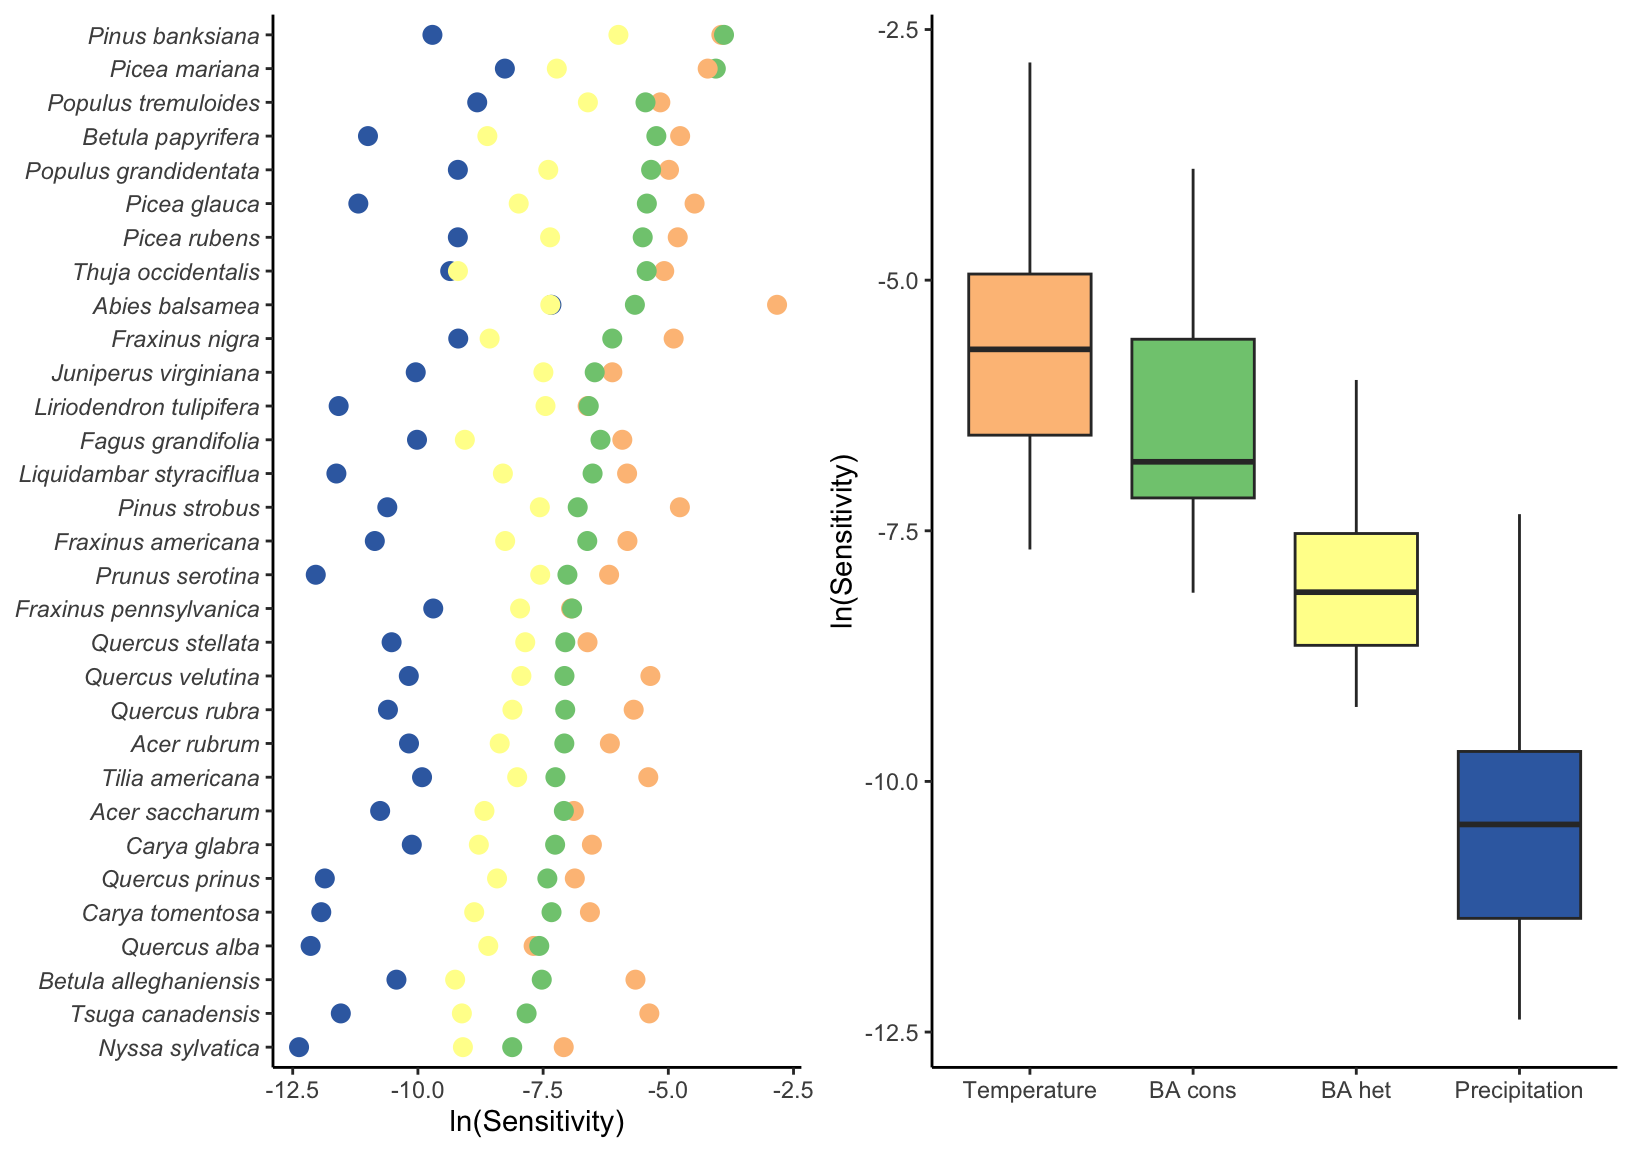
\includegraphics[width=1\textwidth,height=\textheight]{https://willvieira.github.io/book_forest-demography-IPM/marginal_lambda_files/figure-html/fig-ame-1.png}
\caption{Log sensitivity of species population growth rate to
conspecific competition, heterospecific competition, mean annual
temperature, and mean annual precipitation across all plot-year
observations. The smaller the values, the lower the sensitivity to a
covariate.}\label{fig:mean_sens}
}
\end{figure}

We split plots into different regions to ask for each species if
sensitivity to climate and competition changes between cold and hot
portions of the range (Figure \ref{fig:cold_vs_hot}). We evaluate the
sensitivity of each species' border location according to the average
Mean Annual Temperature (MAT) among all plots of the species' border
group. Species distributed toward colder temperature ranges often
exhibited a decrease in sensitivity to climate from the cold to the hot
border. Conversely, most species in the hot range distribution
demonstrated increased sensitivity to climate at the hot border compared
to the cold. Most species also presented a decreased sensitivity to
competition from the cold to the hot border. The decrease in sensitivity
to competition from the cold to the hot border was more pronounced for
boreal species.

\begin{figure}
\hypertarget{fig:cold_vs_hot}{%
\centering
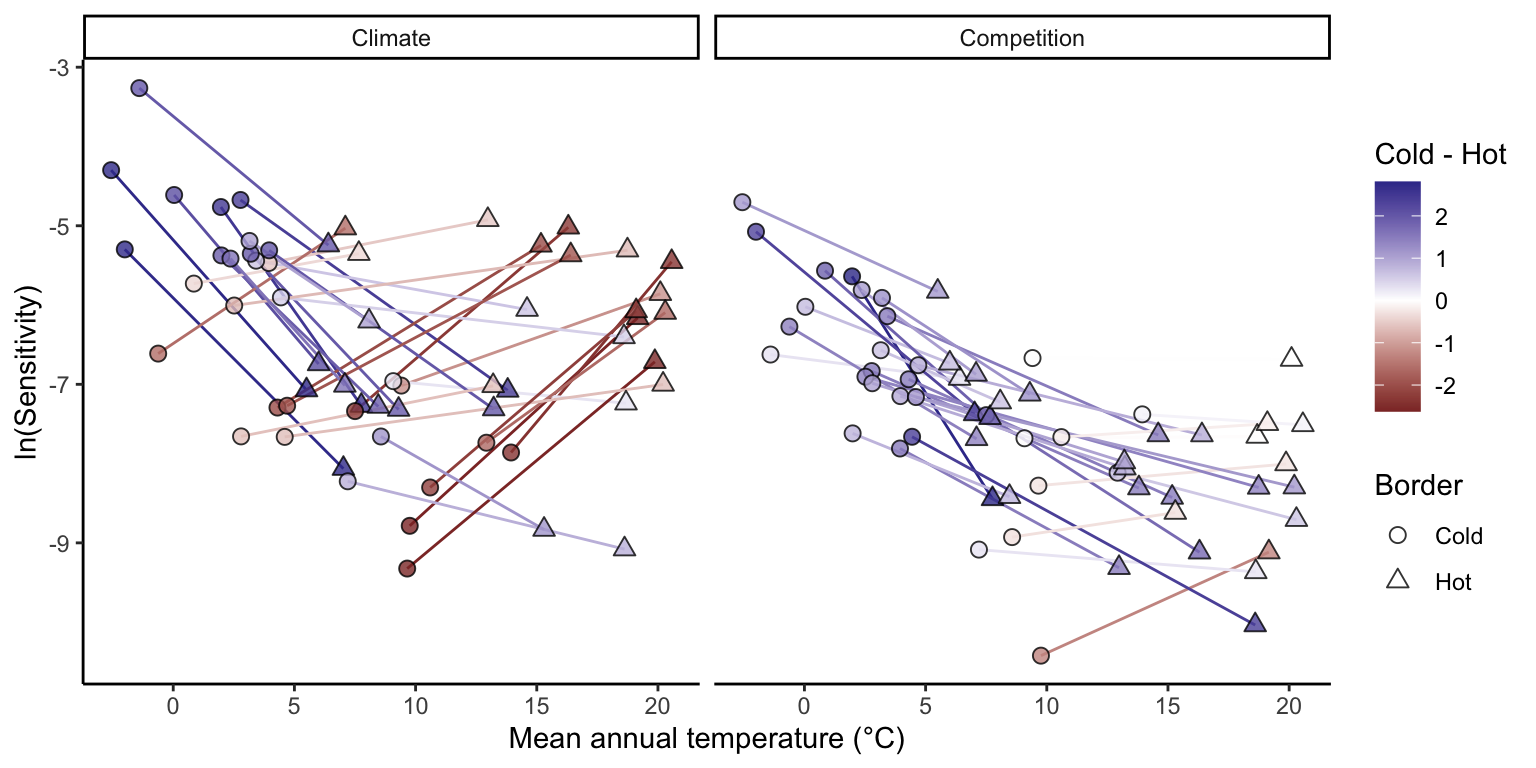
\includegraphics[width=1\textwidth,height=\textheight]{https://willvieira.github.io/book_forest-demography-IPM/marginal_lambda_files/figure-html/fig-hot_vs_cold-1.png}
\caption{Differences in species population growth rate sensitivity to
climate (left) and competition between the cold and hot range limits.
Each species is represented by a connected line linking their cold
(circle) and hot (triangle) range positions, colored according to the
difference between the cold and hot sensitivities. Note that uncertainty
in each sensitivity point estimation has been omitted for
clarity.}\label{fig:cold_vs_hot}
}
\end{figure}

We further explore the relative sensitivity between climate and
competition changes across the species' range distribution (Figure
\ref{fig:temp_vs_comp}). \(\lambda\) was more sensitive to climate than
competition for almost all species across the cold, center, and hot
ranges (\(ln(CCR)\) below zero). Across the MAT range distribution, the
relative effect of climate to competition increased toward both the cold
and hot borders of the range. This indicates that species located at the
extremes of the MAT range distribution are even more sensitive to
climate than species at the center. Interestingly, the reason for this
increase is not the same for the cold and hot ranges. In the cold range,
the sensitivity of \(\lambda\) increased for both climate and
competition but was proportionally larger for climate. Conversely, in
the hot range, the relative sensitivity to climate increased due to a
significant decrease in sensitivity to competition.

\begin{figure}
\hypertarget{fig:temp_vs_comp}{%
\centering
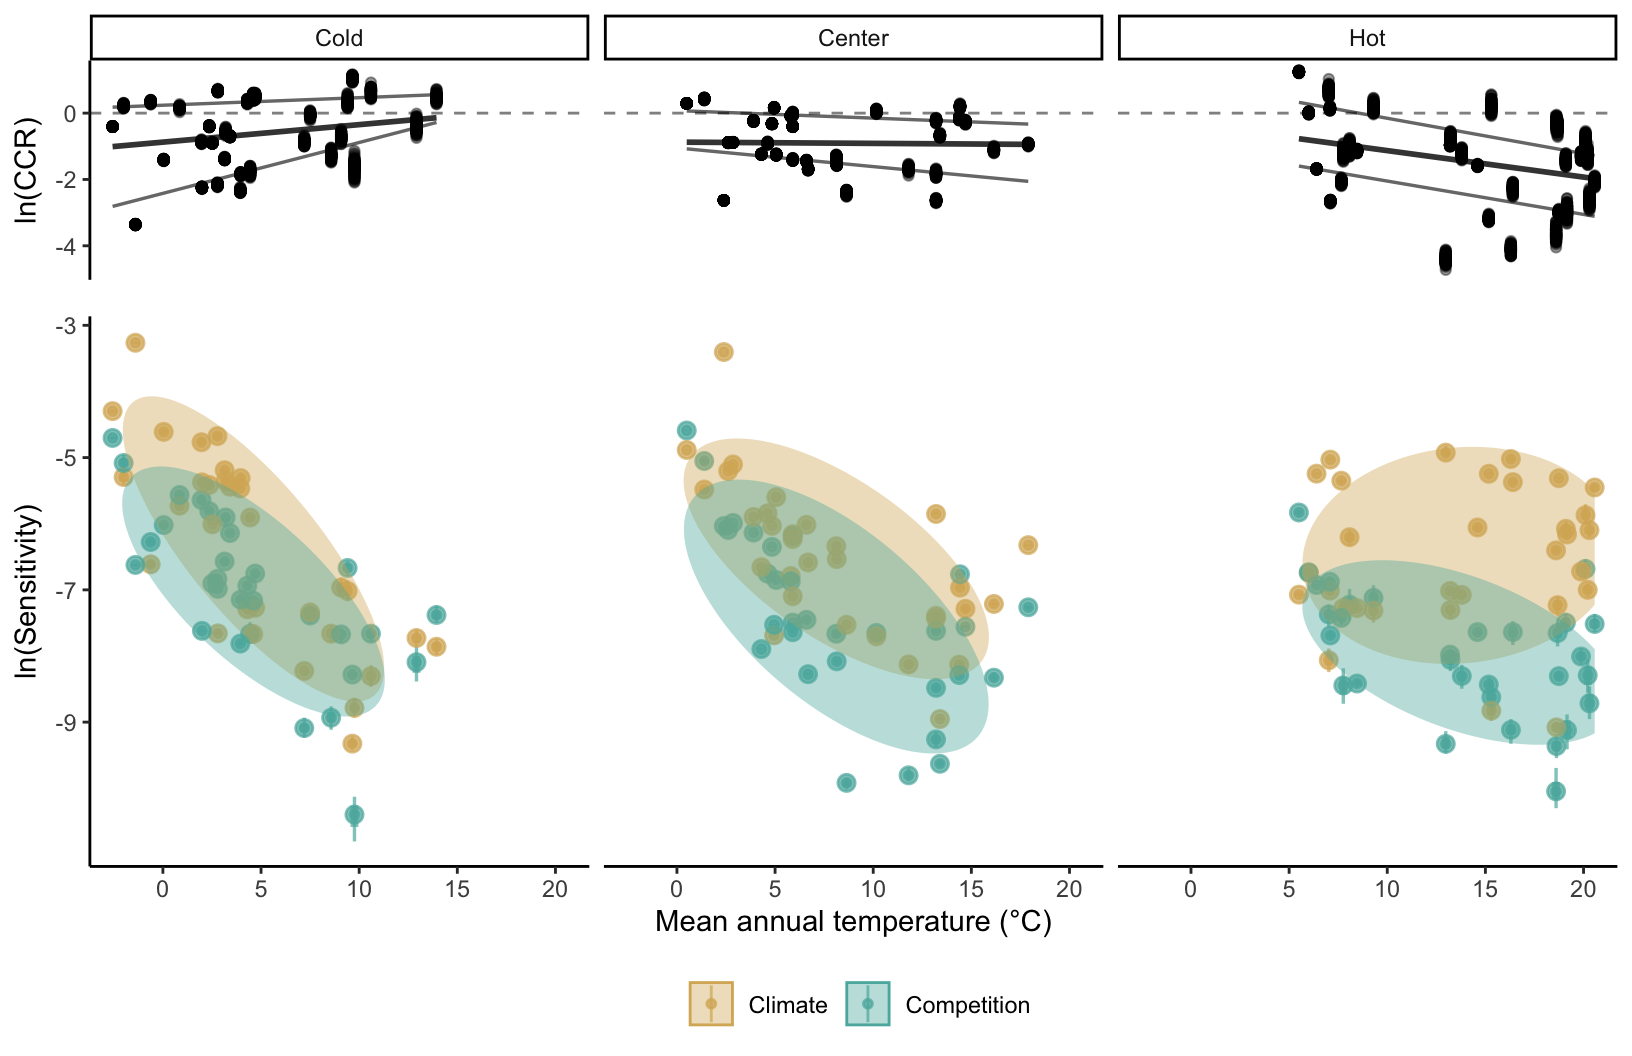
\includegraphics[width=1\textwidth,height=\textheight]{https://willvieira.github.io/book_forest-demography-IPM/marginal_lambda_files/figure-html/fig-sensBorder_temp-1.png}
\caption{Bottom panels describe the sensitivity of species population
growth rate to competition (green) and climate (yellow) across the cold,
center, and hot temperature ranges. The top panels show the log ratio
between competition and climate sensitivities, where negative values
mean climate sensitivity is relatively higher than competition. We
defined each species' temperature range position as the median Mean
Annual Temperature across all observed plots for each cold, center, and
hot range class. In the bottom panel, species points are grouped by a
Multivariate Normal Density function with 75\% probability, while in the
top panel, the lines represent the 25, 50, and 75\% quantile
probabilities.}\label{fig:temp_vs_comp}
}
\end{figure}

\hypertarget{discussion}{%
\section{Discussion}\label{discussion}}

We developed an integral projection model for 31 tree species linking
growth, survival, and recruitment to stand level \(\lambda\) in order to
assess the sensitivity of \(\lambda\) to climate and competition. Our
model advances previous analysis of tree species performance by (i)
explicitly incorporating climate and competition effects in the
recruitment model, (ii) distinguishing between conspecific and
heterospecific competition, while (iii) tracking model's uncertainty at
both the individual and plot levels. Moreover, we designed a modular
approach that is easily extendable to include any of the over 200
available species in the dataset and additional covariates influencing
each demographic rate.

The results reveal that, for all species, adding climate and competition
covariates enhances the predictability of all demographic components in
comparison to a simple random effect model without covariates.
Nevertheless, the most influential variable remained the local plot
conditions captured by the random effects. Therefore, we evaluated
species sensitivity to climate and competition while considering
plot-level variability. Across the species and their respective ranges,
we found that \(\lambda\) was more sensitive to temperature and
conspecific basal area of larger individuals. Furthermore, these
sensitivities were contingent on the range position of the species, with
climate being relatively more important than competition at both the
cold and hot range border. These findings contribute to a better
understanding of how tree species might respond to novel conditions
arising from climate change and perturbations, providing valuable
insights for their management.

\textbf{\emph{Fit of demographic components}}

Our model demonstrated remarkable coherence when reproducing the known
variation in traits related to growth, survival, and recruitment
components found in the literature. The intercepts for growth and
survival were correlated with maximal size and longevity (Burns et al.
\protect\hyperlink{ref-burns1990silvics}{1990}), while the recruitment
intercept aligned well with the seed mass (Díaz et al.
\protect\hyperlink{ref-diaz2022}{2022}). Additionally, the models
effectively reproduced the fast-slow continuum (Salguero-G\a'omez et al.
\protect\hyperlink{ref-SalgueroGomez2016}{2016}), showing a negative
correlation between growth and survival rate and a positive correlation
between growth and recruitment rate (Figure S14). Regarding competition,
the model captured the negative correlation between density dependence
and shade tolerance. The model also matches a common expectation of
communities where species coexist, with a stronger response to
conspecific competition relative to heterospecific competition, crucial
for biodiversity maintenance (Chesson
\protect\hyperlink{ref-Chesson2000a}{2000}). The intensity of
conspecific density dependence was also higher for fast-growing trees
than for slow-growing ones (Figure S15), similar to observations in
tropical trees (Zhu et al. \protect\hyperlink{ref-Zhu2018}{2018}). For
climate, validation is challenging due to limited data on optimal
temperature and precipitation measures. Nevertheless, our results align
with others, indicating the presence of demographic compensation across
forest trees (Bohner and Diez \protect\hyperlink{ref-bohner2020}{2020},
Yang et al. \protect\hyperlink{ref-Yang2022}{2022}). Furthermore, the
estimated breadth of response to climate correlates with the range size
(Figure S16), suggesting that the model captures information not
explicitly included.

Most of the variability in \(\lambda\) was associated with local plot
conditions captured by random effects, akin to previous studies
(Vanderwel et al. \protect\hyperlink{ref-Vanderwel2016a}{2016}, Le Squin
et al. \protect\hyperlink{ref-LeSquin2021}{2021}). This implies the
influence of other determinants of demography beyond climate and
competition. For instance, at a local scale, soil nitrogen content
(Ib\a'añez et al. \protect\hyperlink{ref-Ibanez2018}{2018}) and mixed
mycorrhizal associations (Luo et al.
\protect\hyperlink{ref-Luo2023}{2023}) can enhance growth rates. At
larger scales, events such as wildfires and insect outbreaks play
crucial roles in forest dynamics and stand structure (Franklin et al.
\protect\hyperlink{ref-Franklin2002}{2002}), causing synchronized
mortality and altering stand composition and abundance. While we focused
on quantifying the effect of climate and competition, other covariates
may have greater importance in driving variance in demographic rates.
For instance, tree growth models showed improved estimates when
accounting for extreme climatic events (Sangin\a'es de C\a'arcer et al.
\protect\hyperlink{ref-Sangines2017}{2017}), and unusual drought events,
rather than average precipitation, were the highest predictors of tree
fecundity after temperature (Clark et al.
\protect\hyperlink{ref-Clark2011}{2011}).

\textbf{\emph{\(\lambda\) sensitivity to climate and competition}}

We found that the sensitivity of \(\lambda\) was higher for temperature,
followed by conspecific competition, across the species. Studies
examining the relative impacts of climate and competition on tree
performance yield diverse outcomes. For instance, while some suggest
that competition has a higher effect on growth than climate
(G\a'omez-Aparicio et al.
\protect\hyperlink{ref-GomezAparicio2011}{2011}, Le Squin et al.
\protect\hyperlink{ref-LeSquin2021}{2021}), others find the opposite
(Copenhaver-Parry and Cannon
\protect\hyperlink{ref-CopenhaverParry2016}{2016}). Furthermore, the
relative effect between climate and competition can change between
demographic components, where growth is more sensitive to competition
while fecundity to climate (Clark et al.
\protect\hyperlink{ref-Clark2011}{2011}). This disparity may arise from
a tendency to evaluate sensitivity to specific demographic rates rather
than considering their integrated effects. This is particularly critical
since the population growth rate does not respond equally to all
covariates. We performed additional sensitivity analyses, which revealed
that most species are primarily sensitive to recruitment, followed by
survival, with a relatively lower impact from growth (see Supplementary
Material 3).

Assessing climate sensitivity across the species range distribution
revealed divergent responses. As species' performance changes
nonlinearly with climate, lower sensitivity values to a climate
covariate indicate that the species operates under optimal climate
conditions, whereas higher sensitivity values suggest the species is
deviating from its optimal climate condition. Overall, climate
sensitivity (primarily driven by MAT) was higher at both the cold and
hot range extremes. This implies that species coming from colder
temperatures exhibit optimal performance towards their warmer range, and
vice versa for species from hotter conditions. Interestingly, the
demographic components driving higher sensitivity to climate at the cold
and hot extremes differ. The recruitment and growth models primarily
influenced sensitivity at the cold border, while the survival model
dominated at the hot border (see Figure S17). Previous studies have
indicated climate-constrained growth rates at the cold border for North
American (Ettinger and HilleRisLambers
\protect\hyperlink{ref-Ettinger2013}{2013}) and European (Kunstler et
al. \protect\hyperlink{ref-Kunstler2021}{2021}) trees. Consistent with
our results, a decrease in survival at the hot border was observed for
European trees (Kunstler et al.
\protect\hyperlink{ref-Kunstler2021}{2021}), though not in eastern North
America (Purves \protect\hyperlink{ref-Purves2009}{2009}).

The sensitivity of \(\lambda\) to competition increased almost linearly
toward colder temperatures for most species. Due to the nonlinearity
between species' performance and competition, the sensitivity of
\(\lambda\) to changes in competition decreases as stand density
increases (negative exponential shape). This implies that the observed
decrease in sensitivity to competition toward the hot range results from
an overall increase in stand density (i.e.~competition intensity).
Indeed, biotic interactions are often more critical at the warm range
border (Paquette and Hargreaves
\protect\hyperlink{ref-Paquette2021}{2021}). However, when evaluating
only the growth rate of North American (Ettinger and HilleRisLambers
\protect\hyperlink{ref-Ettinger2013}{2013}) and European (Kunstler et
al. \protect\hyperlink{ref-Kunstler2011a}{2011}) trees, the effect of
competition remains constant across the climate range.

\textbf{\emph{Limitations and Future Perspectives}}

Structured population models, such as the IPM, play a crucial role in
capturing ontogenetic variability within tree population dynamics. While
the growth model inherently considers individual size, the survival and
recruitment models are size-independent. We attempted to incorporate the
widely assumed ``U-shape'' form of mortality rate changes with
individual size (Lines et al. \protect\hyperlink{ref-Lines2010}{2010}),
but it performed worse than the simple random effects one (Figure S6).
Mortality has been observed to increase with individual size (Luo and
Chen \protect\hyperlink{ref-Luo2011}{2011}, Hember et al.
\protect\hyperlink{ref-Hember2017}{2017}), but its significance appears
to manifest only when interacting with climate and competition (Le Squin
et al. \protect\hyperlink{ref-LeSquin2021}{2021}). The challenge in
capturing size dependence in the survival model likely stems from the
lack of information on small individuals (dbh \textless{} 12.7 cm) and
the rarity of larger individuals in datasets, even for extensive forest
inventories (Canham and Murphy
\protect\hyperlink{ref-Canham2017}{2017}). Despite not explicitly
including individual size in the survival model, its indirect influence
is included with the asymmetric competition, where smaller individuals
experience higher competitive pressure. Another limitation of this
model, shared with many models using forest inventory data
(Kunstler2021; Le Squin et al.
\protect\hyperlink{ref-LeSquin2021}{2021}, Guyennon et al.
\protect\hyperlink{ref-Guyennon2023}{2023}), is its focus on adults,
while tree fecundity can be influenced by climate (Clark et al.
\protect\hyperlink{ref-Clark2021}{2021}), and the dynamics of
recruitment may not necessarily align with those of adults (Serra-Diaz
et al. \protect\hyperlink{ref-SerraDiaz2016}{2016}, Wason and Dovciak
\protect\hyperlink{ref-Wason2017}{2017}, but see Canham and Murphy
\protect\hyperlink{ref-Canham2016}{2016}).

The modular nature of our approach makes it easily extensible to include
new species or covariates. For instance, additional covariates such as
water balance or evapotranspiration could be tested to evaluate the
impact of drought-induced mortality (Peng et al.
\protect\hyperlink{ref-Peng2011}{2011}). Furthermore, exploring the
interaction between climate, competition, and individual size can
enhance predictions of demographic rates (Peng et al.
\protect\hyperlink{ref-Peng2011}{2011}, Rollinson et al.
\protect\hyperlink{ref-Rollinson2016}{2016}, Ford et al.
\protect\hyperlink{ref-Ford2017}{2017}, Le Squin et al.
\protect\hyperlink{ref-LeSquin2021}{2021}). An overlooked but
computationally expensive improvement involves jointly fitting the
growth, survival, and recruitment models. This would enable leveraging
ecological knowledge, such as life history tradeoffs, by sharing
information between processes with abundant data (e.g.~growth) and those
with scarce data (e.g.~recruitment). Future steps should focus on better
understanding the variability captured by random effects and translating
it into ecological processes. While we addressed individual and
plot-level model uncertainty, further considerations for other sources
of variability arising from temporal stochasticity in climate and
competition covariates are essential. This will enhance our
understanding of the effects of spatiotemporal variability on species
performance across their range (Holt et al.
\protect\hyperlink{ref-Holt2022}{2022}).

\hypertarget{references}{%
\section*{References}\label{references}}
\addcontentsline{toc}{section}{References}

\hypertarget{refs}{}
\begin{cslreferences}
\leavevmode\hypertarget{ref-bohner2020}{}%
Bohner, T., and J. Diez. 2020. Extensive mismatches between species
distributions and performance and their relationship to functional
traits. Ecology Letters 23:33--44.

\leavevmode\hypertarget{ref-BoucherLalonde2012}{}%
Boucher-Lalonde, V., A. Morin, and D. J. Currie. 2012. How are tree
species distributed in climatic space? A simple and general pattern.
Global Ecology and Biogeography 21:1157--1166.

\leavevmode\hypertarget{ref-Briscoe2019}{}%
Briscoe, N. J., J. Elith, R. Salguero-G\a'omez, J. J. Lahoz-Monfort, J.
S. Camac, K. M. Giljohann, M. H. Holden, B. A. Hradsky, M. R. Kearney,
S. M. McMahon, B. L. Phillips, T. J. Regan, J. R. Rhodes, P. A. Vesk, B.
A. Wintle, J. D. L. Yen, and G. Guillera-Arroita. 2019. Forecasting
species range dynamics with process-explicit models: matching methods to
applications. Ecology Letters 22:1940--1956.

\leavevmode\hypertarget{ref-burns1990silvics}{}%
Burns, R. M., B. H. Honkala, and Others. 1990. Silvics of North America:
1. Conifers; 2. Hardwoods Agriculture Handbook 654. US Department of
Agriculture, Forest Service, Washington, DC.

\leavevmode\hypertarget{ref-Canham2016}{}%
Canham, C. D., and L. Murphy. 2016. The demography of tree species
response to climate: Seedling recruitment and survival. Ecosphere
7:1--16.

\leavevmode\hypertarget{ref-Canham2017}{}%
Canham, C. D., and L. Murphy. 2017. The demography of tree species
response to climate: Sapling and canopy tree survival. Ecosphere 8.

\leavevmode\hypertarget{ref-Caswell2000}{}%
Caswell, H. 2000. Matrix population models. Sinauer Sunderland, MA.

\leavevmode\hypertarget{ref-Chesson2000a}{}%
Chesson, P. 2000. Mechanisms of maintenance of species diversity. Annu.
Rev. Ecol. Syst 31:343--66.

\leavevmode\hypertarget{ref-Clark2021}{}%
Clark, J. S., R. Andrus, M. Aubry-Kientz, Y. Bergeron, M. Bogdziewicz,
D. C. Bragg, D. Brockway, N. L. Cleavitt, S. Cohen, B. Courbaud, R.
Daley, A. J. Das, M. Dietze, T. J. Fahey, I. Fer, J. F. Franklin, C. A.
Gehring, G. S. Gilbert, C. H. Greenberg, Q. Guo, J. HilleRisLambers, I.
Ibanez, J. Johnstone, C. L. Kilner, J. Knops, W. D. Koenig, G. Kunstler,
J. M. LaMontagne, K. L. Legg, J. Luongo, J. A. Lutz, D. Macias, E. J. B.
McIntire, Y. Messaoud, C. M. Moore, E. Moran, J. A. Myers, O. B. Myers,
C. Nunez, R. Parmenter, S. Pearse, S. Pearson, R. Poulton-Kamakura, E.
Ready, M. D. Redmond, C. D. Reid, K. C. Rodman, C. L. Scher, W. H.
Schlesinger, A. M. Schwantes, E. Shanahan, S. Sharma, M. A. Steele, N.
L. Stephenson, S. Sutton, J. J. Swenson, M. Swift, T. T. Veblen, A. V.
Whipple, T. G. Whitham, A. P. Wion, K. Zhu, and R. Zlotin. 2021.
Continent-wide tree fecundity driven by indirect climate effects. Nature
Communications 12:1--11.

\leavevmode\hypertarget{ref-Clark2011}{}%
Clark, J. S., D. M. Bell, M. H. Hersh, and L. Nichols. 2011. Climate
change vulnerability of forest biodiversity: Climate and competition
tracking of demographic rates. Global Change Biology 17:1834--1849.

\leavevmode\hypertarget{ref-CopenhaverParry2016}{}%
Copenhaver-Parry, P. E., and E. Cannon. 2016. The relative influences of
climate and competition on tree growth along montane ecotones in the
Rocky Mountains. Oecologia 182:13--25.

\leavevmode\hypertarget{ref-Csergo2017}{}%
Csergő, A. M., R. Salguero-G\a'omez, O. Broennimann, S. R. Coutts, A.
Guisan, A. L. Angert, E. Welk, I. Stott, B. J. Enquist, B. McGill, J. C.
Svenning, C. Violle, and Y. M. Buckley. 2017. Less favourable climates
constrain demographic strategies in plants.

\leavevmode\hypertarget{ref-diaz2022}{}%
Díaz, S., J. Kattge, J. H. C. Cornelissen, I. J. Wright, S. Lavorel, S.
Dray, B. Reu, M. Kleyer, C. Wirth, I. C. Prentice, and Others. 2022. The
global spectrum of plant form and function: enhanced species-level trait
dataset. Scientific Data 9:755.

\leavevmode\hypertarget{ref-Easterling2000}{}%
Easterling, M. R., S. P. Ellner, and P. M. Dixon. 2000. Size-specific
sensitivity: applying a new structured population model. Ecology
81:694--708.

\leavevmode\hypertarget{ref-Ellner2016}{}%
Ellner, S. P., D. Z. Childs, and M. Rees. 2016. Data-driven modelling of
structured populations. Springer.

\leavevmode\hypertarget{ref-Ettinger2013}{}%
Ettinger, A. K., and J. HilleRisLambers. 2013. Climate isn't everything:
Competitive interactions and variation by life stage will also affect
range shifts in a warming world. American Journal of Botany
100:1344--1355.

\leavevmode\hypertarget{ref-Evans2016}{}%
Evans, M. E. K., C. Merow, S. Record, S. M. McMahon, and B. J. Enquist.
2016. Towards Process-based Range Modeling of Many Species. Trends in
Ecology and Evolution 31:860--871.

\leavevmode\hypertarget{ref-Ford2017}{}%
Ford, K. R., I. K. Breckheimer, J. F. Franklin, J. A. Freund, S. J.
Kroiss, A. J. Larson, E. J. Theobald, and J. HilleRisLambers. 2017.
Competition alters tree growth responses to climate at individual and
stand scales. Canadian Journal of Forest Research 47:53--62.

\leavevmode\hypertarget{ref-Franklin2002}{}%
Franklin, J. F., T. A. Spies, R. V. Pelt, A. B. Carey, D. A. Thornburgh,
D. R. Berg, D. B. Lindenmayer, M. E. Harmon, W. S. Keeton, D. C. Shaw,
K. Bible, and J. Chen. 2002. Disturbances and structural development of
natural forest ecosystems with silvicultural implications, using
Douglas-fir forests as an example. Forest Ecology and Management
155:399--423.

\leavevmode\hypertarget{ref-cmdstanr}{}%
Gabry, J., R. Češnovar, and A. Johnson. 2023. cmdstanr: R Interface to
'CmdStan'.

\leavevmode\hypertarget{ref-Gelman2019}{}%
Gelman, A., B. Goodrich, J. Gabry, and A. Vehtari. 2019. R-squared for
Bayesian Regression Models. American Statistician 73:307--309.

\leavevmode\hypertarget{ref-GomezAparicio2011}{}%
G\a'omez-Aparicio, L., R. García-Vald\a'es, P. Ruíz-Benito, and M. A.
Zavala. 2011. Disentangling the relative importance of climate, size and
competition on tree growth in Iberian forests: Implications for forest
management under global change. Global Change Biology 17:2400--2414.

\leavevmode\hypertarget{ref-Guisan2000}{}%
Guisan, A., and N. E. Zimmermann. 2000. Predictive habitat distribution
models in ecology. Ecological Modelling 135:147--186.

\leavevmode\hypertarget{ref-Guyennon2023}{}%
Guyennon, A., B. Reineking, R. Salguero-Gomez, J. Dahlgren, A. Lehtonen,
S. Ratcliffe, P. Ruiz-Benito, M. A. Zavala, and G. Kunstler. 2023.
Beyond mean fitness: Demographic stochasticity and resilience matter at
tree species climatic edges. Global Ecology and Biogeography
32:573--585.

\leavevmode\hypertarget{ref-Hember2017}{}%
Hember, R. A., W. A. Kurz, and N. C. Coops. 2017. Relationships between
individual-tree mortality and water-balance variables indicate positive
trends in water stress-induced tree mortality across North America.
Global Change Biology 23:1691--1710.

\leavevmode\hypertarget{ref-Holt2009}{}%
Holt, R. D. 2009. Bringing the Hutchinsonian niche into the 21st
century: Ecological and evolutionary perspectives. Proceedings of the
National Academy of Sciences 106:19659--19665.

\leavevmode\hypertarget{ref-Holt2022}{}%
Holt, R. D., M. Barfield, and J. H. Peniston. 2022. Temporal variation
may have diverse impacts on range limits. Philosophical Transactions of
the Royal Society B: Biological Sciences 377.

\leavevmode\hypertarget{ref-Hutchinson1957}{}%
Hutchinson, G. E. 1957. Concluding remarks. Pages 415--427 \emph{in}
Cold spring harbor symposium on quantitative biology.

\leavevmode\hypertarget{ref-Ibanez2018}{}%
Ib\a'añez, I., D. R. Zak, A. J. Burton, and K. S. Pregitzer. 2018.
Anthropogenic nitrogen deposition ameliorates the decline in tree growth
caused by a drier climate. Ecology.

\leavevmode\hypertarget{ref-kohyama1992}{}%
Kohyama, T. 1992. Size-structured multi-species model of rain forest
trees. Functional Ecology:206--212.

\leavevmode\hypertarget{ref-Kunstler2011a}{}%
Kunstler, G., C. H. Albert, B. Courbaud, S. Lavergne, W. Thuiller, G.
Vieilledent, N. E. Zimmermann, and D. A. Coomes. 2011. Effects of
competition on tree radial-growth vary in importance but not in
intensity along climatic gradients. Journal of Ecology 99:300--312.

\leavevmode\hypertarget{ref-Kunstler2021}{}%
Kunstler, G., A. Guyennon, S. Ratcliffe, N. Rüger, P. Ruiz-Benito, D. Z.
Childs, J. Dahlgren, A. Lehtonen, W. Thuiller, C. Wirth, M. A. Zavala,
and R. Salguero-Gomez. 2021. Demographic performance of European tree
species at their hot and cold climatic edges. Journal of Ecology
109:1041--1054.

\leavevmode\hypertarget{ref-LeSquin2021}{}%
Le Squin, A., I. Boulangeat, and D. Gravel. 2021. Climate-induced
variation in the demography of 14 tree species is not sufficient to
explain their distribution in eastern North America. Global Ecology and
Biogeography 30:352--369.

\leavevmode\hypertarget{ref-Lines2010}{}%
Lines, E. R., D. A. Coomes, and D. W. Purves. 2010. Influences of forest
structure, climate and species composition on tree mortality across the
Eastern US. PLoS ONE 5.

\leavevmode\hypertarget{ref-Louthan2015}{}%
Louthan, A. M., D. F. Doak, and A. L. Angert. 2015. Where and When do
Species Interactions Set Range Limits? Trends in Ecology and Evolution
30:780--792.

\leavevmode\hypertarget{ref-Luo2023}{}%
Luo, S., R. P. Phillips, I. Jo, S. Fei, J. Liang, B. Schmid, and N.
Eisenhauer. 2023. Higher productivity in forests with mixed mycorrhizal
strategies. Nature Communications 14:1--10.

\leavevmode\hypertarget{ref-Luo2011}{}%
Luo, Y., and H. Y. H. Chen. 2011. Competition, species interaction and
ageing control tree mortality in boreal forests. Journal of Ecology
99:1470--1480.

\leavevmode\hypertarget{ref-maguire1973niche}{}%
Maguire Jr, B. 1973. Niche response structure and the analytical
potentials of its relationship to the habitat. The American Naturalist
107:213--246.

\leavevmode\hypertarget{ref-McGill2012}{}%
McGill, B. J. 2012. Trees are rarely most abundant where they grow best.
Journal of Plant Ecology 5:46--51.

\leavevmode\hypertarget{ref-McKenney2011}{}%
McKenney, D. W., M. F. Hutchinson, P. Papadopol, K. Lawrence, J. Pedlar,
K. Campbell, E. Milewska, R. F. Hopkinson, D. Price, and T. Owen. 2011.
Customized Spatial Climate Models for North America. Bulletin of the
American Meteorological Society 92:1611--1622.

\leavevmode\hypertarget{ref-Merow2014}{}%
Merow, C., A. M. Latimer, A. M. Wilson, S. M. Mcmahon, A. G. Rebelo, and
J. A. Silander. 2014. On using integral projection models to generate
demographically driven predictions of species' distributions:
Development and validation using sparse data. Ecography 37:1167--1183.

\leavevmode\hypertarget{ref-Midolo2021}{}%
Midolo, G., C. Wellstein, and S. Faurby. 2021. Individual fitness is
decoupled from coarse-scale probability of occurrence in North American
trees. Ecography 44:789--801.

\leavevmode\hypertarget{ref-MilnerGulland2017a}{}%
Milner-Gulland, E. J., and K. Shea. 2017. Embracing uncertainty in
applied ecology. Journal of Applied Ecology.

\leavevmode\hypertarget{ref-Naturelles2016}{}%
Minist\a`ere des Ressources Naturelles. 2016. Norme d'inventaire
ecoforestier: placettes-echantillons temporaires. Direction des
inventaires forestier, Ministère des Ressources naturelles,Québec.

\leavevmode\hypertarget{ref-OConnell2007}{}%
O'Connell, M. B., E. B. LaPoint, J. A. Turner, T. Ridley, D. Boyer, A.
Wilson, K. L. Waddell, and B. L. Conkling. 2007. The forest inventory
and analysis database: Database description and users forest inventory
and analysis program. US Department of Agriculture, Forest Service.

\leavevmode\hypertarget{ref-Ohse2023}{}%
Ohse, B., A. Compagnoni, C. E. Farrior, S. M. McMahon, R.
Salguero-G\a'omez, N. Rüger, and T. M. Knight. 2023. Demographic
synthesis for global tree species conservation. Trends in Ecology and
Evolution 38:579--590.

\leavevmode\hypertarget{ref-Pacala1996a}{}%
Pacala, S. W., C. D. Canham, J. Saponara, J. A. Silander, R. K. Kobe, E.
Ribbens, J. A. S. Jr., R. K. Kobe, and E. Ribbens. 1996. Forest models
defined by Field Measurements: Estimation, Error Analysis and Dynamics.
Ecological Monographs 66:1--43.

\leavevmode\hypertarget{ref-Pagel2012}{}%
Pagel, J., and F. M. Schurr. 2012. Forecasting species ranges by
statistical estimation of ecological niches and spatial population
dynamics. Global Ecology and Biogeography 21:293--304.

\leavevmode\hypertarget{ref-Paquette2021}{}%
Paquette, A., and A. L. Hargreaves. 2021. Biotic interactions are more
often important at species' warm versus cool range edges. Ecology
Letters 24:2427--2438.

\leavevmode\hypertarget{ref-Peng2011}{}%
Peng, C., Z. Ma, X. Lei, Q. Zhu, H. Chen, W. Wang, S. Liu, W. Li, X.
Fang, and X. Zhou. 2011. A drought-induced pervasive increase in tree
mortality across Canada's boreal forests. Nature Climate Change
1:467--471.

\leavevmode\hypertarget{ref-Pulliam2000}{}%
Pulliam, H. R. 2000. On the relationship between niche and distribution.
Ecology Letters 3:349--361.

\leavevmode\hypertarget{ref-Purves2009}{}%
Purves, D. W. 2009. The demography of range boundaries versus range
cores in eastern US tree species. Proceedings of the Royal Society B:
Biological Sciences 276:1477--1484.

\leavevmode\hypertarget{ref-Reich1998}{}%
Reich, P. B., M. G. Tjoelker, M. B. Walters, D. W. Vanderklein, and C.
Buschena. 1998. Close association of RGR, leaf and root morphology, seed
mass and shade tolerance in seedlings of nine boreal tree species grown
in high and low light. Functional Ecology 12:327--338.

\leavevmode\hypertarget{ref-Rollinson2016}{}%
Rollinson, C. R., M. W. Kaye, and C. D. Canham. 2016. Interspecific
variation in growth responses to climate and competition of five eastern
tree species. Ecology 97:1003--1011.

\leavevmode\hypertarget{ref-Russell2012}{}%
Russell, B. D., C. D. G. Harley, T. Wernberg, N. Mieszkowska, S.
Widdicombe, J. M. Hall-Spencer, and S. D. Connell. 2012. Predicting
ecosystem shifts requires new approaches that integrate the effects of
climate change across entire systems. Biology Letters 8:164--166.

\leavevmode\hypertarget{ref-SalgueroGomez2016}{}%
Salguero-G\a'omez, R., O. R. Jones, E. Jongejans, S. P. Blomberg, D. J.
Hodgson, C. Mbeau-Ache, P. A. Zuidema, H. De Kroon, and Y. M. Buckley.
2016. Fast--slow continuum and reproductive strategies structure plant
life-history variation worldwide. Proceedings of the National Academy of
Sciences 113:230--235.

\leavevmode\hypertarget{ref-Sangines2017}{}%
Sangin\a'es de C\a'arcer, P., Y. Vitasse, J. Peñuelas, V. E. J. Jassey,
A. Buttler, and C. Signarbieux. 2017. Vapor-pressure deficit and extreme
climatic variables limit tree growth. Global Change Biology
12:3218--3221.

\leavevmode\hypertarget{ref-Scherrer2020}{}%
Scherrer, D., Y. Vitasse, A. Guisan, T. Wohlgemuth, and H. Lischke.
2020. Competition and demography rather than dispersal limitation slow
down upward shifts of trees' upper elevation limits in the Alps. Journal
of Ecology:1--15.

\leavevmode\hypertarget{ref-SerraDiaz2016}{}%
Serra-Diaz, J. M., J. Franklin, W. W. Dillon, A. D. Syphard, F. W.
Davis, and R. K. Meentemeyer. 2016. California forests show early
indications of both range shifts and local persistence under climate
change. Global Ecology and Biogeography 25:164--175.

\leavevmode\hypertarget{ref-Sittaro2017}{}%
Sittaro, F., A. Paquette, C. Messier, and C. A. Nock. 2017. Tree range
expansion in eastern North America fails to keep pace with climate
warming at northern range limits. Global Change Biology:1--10.

\leavevmode\hypertarget{ref-Svenning2014}{}%
Svenning, J.-C. C., D. Gravel, R. D. Holt, F. M. Schurr, W. Thuiller, T.
Münkemüller, K. H. Schiffers, S. Dullinger, T. C. Edwards, T. Hickler,
S. I. Higgins, J. E. M. S. Nabel, J. Pagel, and S. Normand. 2014. The
influence of interspecific interactions on species range expansion
rates. Ecography 37:1198--1209.

\leavevmode\hypertarget{ref-Talluto2017}{}%
Talluto, M. V., I. Boulangeat, S. Vissault, W. Thuiller, and D. Gravel.
2017. Extinction debt and colonization credit delay range shifts of
eastern North American trees. Nature Ecology \& Evolution 1:0182.

\leavevmode\hypertarget{ref-stan2022stan}{}%
Team, S. D., and Others. 2022. Stan modeling language users guide and
reference manual, version 2.30.1. Stan Development Team.

\leavevmode\hypertarget{ref-thomas2004}{}%
Thomas, C. D., A. Cameron, R. E. Green, M. Bakkenes, L. J. Beaumont, Y.
C. Collingham, B. F. N. Erasmus, M. F. De Siqueira, A. Grainger, L.
Hannah, and Others. 2004. Extinction risk from climate change. Nature
427:145--148.

\leavevmode\hypertarget{ref-Thuiller2014}{}%
Thuiller, W., T. Munkemuller, K. H. Schiffers, D. Georges, S. Dullinger,
V. M. Eckhart, T. C. Edwards, D. Gravel, G. Kunstler, C. Merow, K.
Moore, C. Piedallu, S. Vissault, N. E. Zimmermann, D. Zurell, F. M.
Schurr, T. Münkemüller, K. H. Schiffers, D. Georges, S. Dullinger, V. M.
Eckhart, T. C. Edwards, D. Gravel, G. Kunstler, C. Merow, K. Moore, C.
Piedallu, S. Vissault, N. E. Zimmermann, D. Zurell, and F. M. Schurr.
2014. Does probability of occurrence relate to population dynamics?
Ecography 37:1155--1166.

\leavevmode\hypertarget{ref-Tredennick2021}{}%
Tredennick, A. T., G. Hooker, S. P. Ellner, and P. B. Adler. 2021. A
practical guide to selecting models for exploration, inference, and
prediction in ecology. Ecology 102:e03336.

\leavevmode\hypertarget{ref-Vanderwel2016a}{}%
Vanderwel, M. C., H. Zeng, J. P. Caspersen, G. Kunstler, and J. W.
Lichstein. 2016. Demographic controls of aboveground forest biomass
across North America. Ecology Letters 19:414--423.

\leavevmode\hypertarget{ref-Villellas2015}{}%
Villellas, J., D. F. Doak, M. B. García, and W. F. Morris. 2015.
Demographic compensation among populations: What is it, how does it
arise and what are its implications? Ecology Letters 18:1139--1152.

\leavevmode\hypertarget{ref-von1957quantitative}{}%
Von Bertalanffy, L. 1957. Quantitative laws in metabolism and growth.
The quarterly review of biology 32:217--231.

\leavevmode\hypertarget{ref-Wason2017}{}%
Wason, J. W., and M. Dovciak. 2017. Tree demography suggests multiple
directions and drivers for species range shifts in mountains of
Northeastern United States. Global Change Biology 23:3335--3347.

\leavevmode\hypertarget{ref-Yang2022}{}%
Yang, X., A. L. Angert, P. A. Zuidema, F. He, S. Huang, S. Li, S. L. Li,
N. I. Chardon, and J. Zhang. 2022. The role of demographic compensation
in stabilising marginal tree populations in North America. Ecology
Letters 25:1676--1689.

\leavevmode\hypertarget{ref-Zhang2015}{}%
Zhang, J., S. Huang, and F. He. 2015. Half-century evidence from western
Canada shows forest dynamics are primarily driven by competition
followed by climate. Proceedings of the National Academy of Sciences
112:4009--4014.

\leavevmode\hypertarget{ref-Zhu2012}{}%
Zhu, K., C. W. Woodall, and J. S. Clark. 2012. Failure to migrate: Lack
of tree range expansion in response to climate change. Global Change
Biology 18:1042--1052.

\leavevmode\hypertarget{ref-Zhu2018}{}%
Zhu, Y., S. A. Queenborough, R. Condit, S. P. Hubbell, K. P. Ma, and L.
S. Comita. 2018. Density-dependent survival varies with species
life-history strategy in a tropical forest. Ecology Letters.

\leavevmode\hypertarget{ref-zuidema2010integral}{}%
Zuidema, P. A., E. Jongejans, P. D. Chien, H. J. During, and F.
Schieving. 2010. Integral projection models for trees: a new
parameterization method and a validation of model output. Journal of
Ecology 98:345--355.
\end{cslreferences}


\newpage


\end{document}